\documentclass[journal]{IEEEtran}

\usepackage[utf8]{inputenc}
\usepackage[T1]{fontenc}
\usepackage{amsmath,amssymb}
\usepackage{graphicx}
\usepackage{booktabs}
\usepackage{multirow}
\usepackage{array}
\usepackage{tabularx}
\usepackage{url}
\usepackage{xcolor}
\usepackage{cite}
\usepackage{subcaption}
\usepackage{listings}
\usepackage{enumitem}
\usepackage{seqsplit}
\usepackage[hidelinks]{hyperref}

\graphicspath{{../results/images/}{../results/}{images/}{figures/}}

\newcolumntype{Y}{>{\raggedright\arraybackslash}X}
\newcommand{\mf}{Macro-F1}
\newcommand{\wf}{Weighted-F1}
\newcommand{\acc}{Accuracy}
\newcommand{\model}[1]{\texttt{#1}}

\lstdefinestyle{code}{
  basicstyle=\ttfamily\footnotesize,
  breaklines=true,
  frame=single,
  columns=fullflexible,
  keepspaces=true,
  xleftmargin=1mm,
  xrightmargin=1mm
}

\title{Reimplementation and Improvement of ViHateT5 for Vietnamese Hate Speech Detection}

\author{
  \textbf{Phat Nguyen Cong}$^{1,2}$, \textbf{An Truong Hoang Thanh}$^{1,2}$, \textbf{Cuong Vu Viet}$^{1,2}$ \\
  \addlinespace[0.2cm]
  $^1$University of Information Technology, Ho Chi Minh City, Vietnam \\
  $^2$Vietnam National University, Ho Chi Minh City, Vietnam \\
  \texttt{\{23521143, 23520032, 23520213\}@gm.uit.edu.vn} \\
  \addlinespace[0.1cm]
  \textit{Supervisor: Dr. Ha Minh Tan}
}

\begin{document}
\maketitle

\begin{abstract}
Vietnamese hate speech detection is challenging because harmful online content contains slang, teencode, misspellings, implicit attacks, sarcasm, and severe class imbalance. This report presents an IEEE-style reimplementation and extension of ViHateT5, a unified text-to-text transformer framework for Vietnamese hate speech detection. We reproduce the main pipeline of the original paper: automatic labeling of a large VOZ forum corpus, continual domain pre-training of ViT5 with span corruption, and multi-task sequence-to-sequence fine-tuning on ViHSD, ViCTSD, and ViHOS. We also evaluate BERT-based baselines and several improvements, including Focal Loss, Easy Data Augmentation (EDA), back-translation, weighted ensemble, per-class error analysis, and McNemar statistical testing. Our best balanced ViHateT5-style variant reaches an average \mf{} of 0.7501 across the three downstream datasets. The Focal Loss experiment reaches 0.7478 \mf{} on ViHSD, but it is not the best average model across all datasets. The results show that domain-specific pre-training on Vietnamese forum/social-media data is the key factor, while loss reweighting and ensemble methods are useful but limited unless model errors are complementary.
\end{abstract}

\begin{IEEEkeywords}
Vietnamese hate speech detection, ViHateT5, ViT5, text-to-text learning, span corruption, focal loss, data augmentation, ensemble learning, social media NLP.
\end{IEEEkeywords}

\section{Introduction}
The rapid growth of Vietnamese user-generated content has made online moderation increasingly difficult. Hate speech, toxic language, and offensive expressions appear in social networks, video platforms, forums, and short informal conversations. Unlike formal Vietnamese documents, online comments often contain non-standard spelling, teencode, mixed languages, emojis, abbreviations, sarcasm, and context-dependent references. These characteristics make keyword-based filtering unreliable and make manual moderation infeasible at scale.

Vietnamese hate speech detection (HSD) is not a single task. ViHSD formulates HSD as three-way sentence classification with CLEAN, OFFENSIVE, and HATE labels. ViCTSD uses a binary toxic-speech formulation. ViHOS focuses on span detection, where a model must identify the exact toxic or hateful fragments inside a sentence. A practical system should ideally support all of these tasks without maintaining a separate architecture and prediction head for each dataset.

ViHateT5 \cite{vihatet5} addresses this fragmentation by casting Vietnamese HSD tasks into a unified text-to-text framework. Instead of attaching a task-specific classification head to an encoder, the model receives a task prefix and generates the expected output as text. For sentence classification, the generated text is a label. For span detection, the generated text contains marked hateful spans. The original work also introduces a large VOZ-HSD corpus and performs continual pre-training to adapt ViT5 \cite{vit5} to the social-media/forum domain.

This project has two goals. First, we reimplement the main ViHateT5 pipeline under realistic student-project constraints. Second, we analyze and improve the pipeline with data-centric and model-centric strategies. Our contributions are:
\begin{itemize}[leftmargin=*]
  \item A reimplementation of the auto-labeling, domain pre-training, multi-task fine-tuning, and evaluation pipeline for Vietnamese HSD.
  \item A comparison between text-to-text models and encoder-only BERT-style baselines.
  \item Four improvement directions: Focal Loss, EDA augmentation, back-translation augmentation, and weighted ensemble.
  \item A detailed error analysis with confusion matrices, per-class reports, and McNemar statistical tests.
  \item A deployed demo system and a reproducible repository with trained models and result artifacts.
\end{itemize}

The rest of this report follows the required IEEE journal style. Section II reviews related work. Section III describes the datasets. Section IV presents the methodology. Section V analyzes representative test cases and preprocessing formats. Sections VI and VII report experiments and results. Section VIII analyzes errors. Sections IX and X describe the demo system and limitations. Section XI concludes the report.

\section{Related Work}
\subsection{Hate Speech Detection}
Hate speech detection has been widely studied for English and multilingual social-media text. HateBERT \cite{hatebert}, for example, adapts BERT to abusive language by retraining it on Reddit discussions. The main intuition is that a model trained on general text may not understand abusive language, slang, and social-media discourse. This intuition is directly relevant to Vietnamese because harmful comments often use informal spelling, teencode, and implicit insults.

\subsection{Vietnamese Language Models}
PhoBERT \cite{phobert} is a strong Vietnamese encoder-only model based on RoBERTa. ViSoBERT \cite{visobert} is designed for Vietnamese social-media text and is therefore suitable for labeling VOZ comments. However, BERT-style models are naturally encoder-only. They usually produce a vector representation followed by a classification head, which is efficient but less flexible when multiple output formats are required.

Text-to-text models solve this issue by making the output space textual. T5 \cite{t5} showed that many NLP tasks can be unified as text-to-text transfer learning. mT5 \cite{mt5} extends this idea to many languages, while ViT5 \cite{vit5} specializes the T5 architecture for Vietnamese. ViHateT5 builds on ViT5 and adds continual pre-training on HSD-domain data, making it more suitable for Vietnamese harmful-content detection.

\subsection{Vietnamese HSD Datasets}
ViHSD \cite{vihsd}, ViCTSD \cite{victsd}, and ViHOS \cite{vihos} represent different aspects of harmful language detection. ViHSD is a three-class sentence-level task. ViCTSD is a binary toxic-speech task. ViHOS is a span-level dataset, making it closer to extractive detection than ordinary classification. The diversity of these datasets motivates a unified architecture.

\subsection{Position of This Work}
The original ViHateT5 paper reports strong results and proposes a unified model. Our work does not claim a new architecture. Instead, it provides an independent reimplementation, a clearer engineering analysis, and controlled improvements. This distinction is important: some improvements, such as Focal Loss, help a specific dataset but do not automatically improve the average score across all downstream tasks.

\section{Datasets}
\subsection{Dataset Overview}
Table \ref{tab:datasets} summarizes the four datasets used in the pipeline. The three downstream datasets are used for supervised fine-tuning and evaluation. VOZ-HSD is used for continual domain pre-training after automatic labeling.

\begin{table}[!t]
\centering
\caption{Datasets used in the project.}
\label{tab:datasets}
\resizebox{\columnwidth}{!}{%
\begin{tabular}{llll}
\toprule
\textbf{Dataset} & \textbf{Task Type} & \textbf{Labels/Output} & \textbf{Role} \\
\midrule
ViHSD & Sentence classification & CLEAN/OFFENSIVE/HATE & Downstream \\
ViCTSD & Binary classification & NONE/TOXIC & Downstream \\
ViHOS & Span detection & Hate spans & Downstream \\
VOZ-HSD & Forum corpus & Auto-labeled & Pre-training \\
\bottomrule
\end{tabular}}
\end{table}

\subsection{Downstream Datasets}
ViHSD contains roughly 33,400 comments collected from Vietnamese social-media platforms. It is highly imbalanced: CLEAN dominates, while HATE is a minority class. This motivates the use of \mf{} rather than accuracy as the main metric.

ViCTSD contains around 10,000 samples for binary toxic speech detection. The task is simpler than ViHSD because it contains only two labels, but toxic language still varies by context and register.

ViHOS contains hate span annotations. Unlike ViHSD and ViCTSD, ViHOS requires the model to identify the toxic segment rather than only assign a sentence label. This makes evaluation more sensitive: a prediction can be semantically close but still lose score if the span boundary is incorrect.

\begin{table*}[!t]
\centering
\caption{Detailed characteristics of the three downstream HSD datasets.}
\label{tab:downstream_detail}
\begin{tabular}{lccc}
\toprule
\textbf{Characteristic} & \textbf{ViHSD} & \textbf{ViCTSD} & \textbf{ViHOS} \\
\midrule
Data source & Facebook, YouTube & News, social media & Vietnamese social media \\
Scale & 33,400 comments & 10,000 samples & 11,056 comments \\
Label format & CLEAN / OFFENSIVE / HATE & NONE / TOXIC & Span-level [HATE] \\
Split & Train 80\%, Dev 10\%, Test 10\% & Train 70\%, Dev 15\%, Test 15\% & Dataset-defined split \\
Imbalance & CLEAN $\approx$ 80\%, HATE $\approx$ 5\% & NONE $\approx$ 80\%, TOXIC $\approx$ 20\% & $>$26,000 toxic spans \\
Task type & Sentence classification & Binary classification & Span detection \\
Main metric & Macro-F1 & Macro-F1 & Macro-F1 \\
Difficulty & Medium & Easier & Hard \\
\bottomrule
\end{tabular}
\end{table*}

Table \ref{tab:downstream_detail} clarifies why a unified model is useful. The datasets are not just different in size; they require different prediction formats. ViHSD and ViCTSD can be treated as label generation tasks, while ViHOS requires span-sensitive output. This difference also explains why augmentation is applied only to ViHSD and ViCTSD: random textual changes can break token-level or character-level span annotations in ViHOS.

\subsection{VOZ-HSD and Auto-labeled Data}
The VOZ-HSD corpus contains more than 10 million Vietnamese forum comments. Such scale is valuable for domain adaptation, but the raw corpus is not fully manually labeled. Therefore, the pipeline uses an automatic labeling step to identify hate/offensive comments and construct pre-training subsets. In our reimplementation, ViSoBERT is selected as the auto-labeling model because it is pre-trained on Vietnamese social-media text.

\begin{table}[!t]
\centering
\caption{Label distribution after automatic labeling of VOZ-HSD.}
\label{tab:vozdist}
\begin{tabular}{lrr}
\toprule
\textbf{Label} & \textbf{Samples} & \textbf{Ratio} \\
\midrule
Clean & 10,223,138 & 95.12\% \\
Hate/Offensive & 524,595 & 4.88\% \\
\midrule
Total & 10,747,733 & 100\% \\
\bottomrule
\end{tabular}
\end{table}

Table \ref{tab:vozdist} shows why sampling strategy matters. A full corpus contains more data, but the harmful signal is diluted by the dominant clean class. Balanced sampling increases the relative presence of harmful patterns, while hate-only sampling focuses entirely on harmful language but may reduce the model's ability to contrast harmful and benign comments.

\begin{table*}[!t]
\centering
\caption{VOZ comment distribution by parent thread/topic.}
\label{tab:voz_topics}
\begin{tabular}{clrrr}
\toprule
\textbf{No.} & \textbf{Parent Thread / Topic} & \textbf{Threads} & \textbf{Comments} & \textbf{Size} \\
\midrule
1 & Random conversation & 142,387 & 6,104,792 & 945MB \\
2 & News & 76,107 & 2,030,315 & 304MB \\
3 & Sports & 10,121 & 1,154,658 & 144MB \\
4 & Cars & 12,348 & 552,717 & 96MB \\
5 & Movies -- Music -- Books & 6,467 & 329,601 & 52MB \\
6 & Bikes & 5,093 & 258,728 & 41MB \\
7 & Fashion & 1,845 & 137,548 & 19MB \\
8 & Food -- Travel & 3,492 & 136,649 & 19MB \\
9 & Other hobbies & 690 & 42,737 & 6MB \\
\midrule
& \textbf{Total} & \textbf{258,550} & \textbf{10,747,745} & \textbf{1.66GB} \\
\bottomrule
\end{tabular}
\end{table*}

Table \ref{tab:voz_topics} expands the VOZ-HSD description. The corpus is not a narrow benchmark; it covers random discussion, news, sports, vehicles, entertainment, lifestyle, and other hobbies. The random-conversation category alone contains more than 6.1 million comments, accounting for approximately 56.8\% of the corpus. This category is especially valuable for HSD pre-training because free-form discussion is where slang, teencode, insults, jokes, memes, and implicit toxic expressions frequently appear. The topical diversity also helps the model avoid overfitting to one narrow domain.

\subsection{Dataset Risks}
The datasets introduce several risks. First, label definitions differ across datasets. OFFENSIVE in ViHSD is not identical to TOXIC in ViCTSD, and span labels in ViHOS require a different output format. Second, class imbalance changes how scores should be read. Accuracy can be misleading when CLEAN dominates. Third, informal Vietnamese changes quickly over time; a model trained on one crawl may not fully capture new slang or coded insults.

\section{Methodology}
\subsection{Overall Pipeline}
The system consists of four connected stages. First, we train or select a BERT-style model for automatic labeling. Second, we use the labeled VOZ-HSD corpus to construct hate-only and balanced subsets. Third, we continue pre-training ViT5-base with the T5 span-corruption objective. Fourth, we fine-tune the resulting checkpoint on ViHSD, ViCTSD, and ViHOS in a unified multi-task text-to-text format.

\begin{figure*}[!t]
\centering
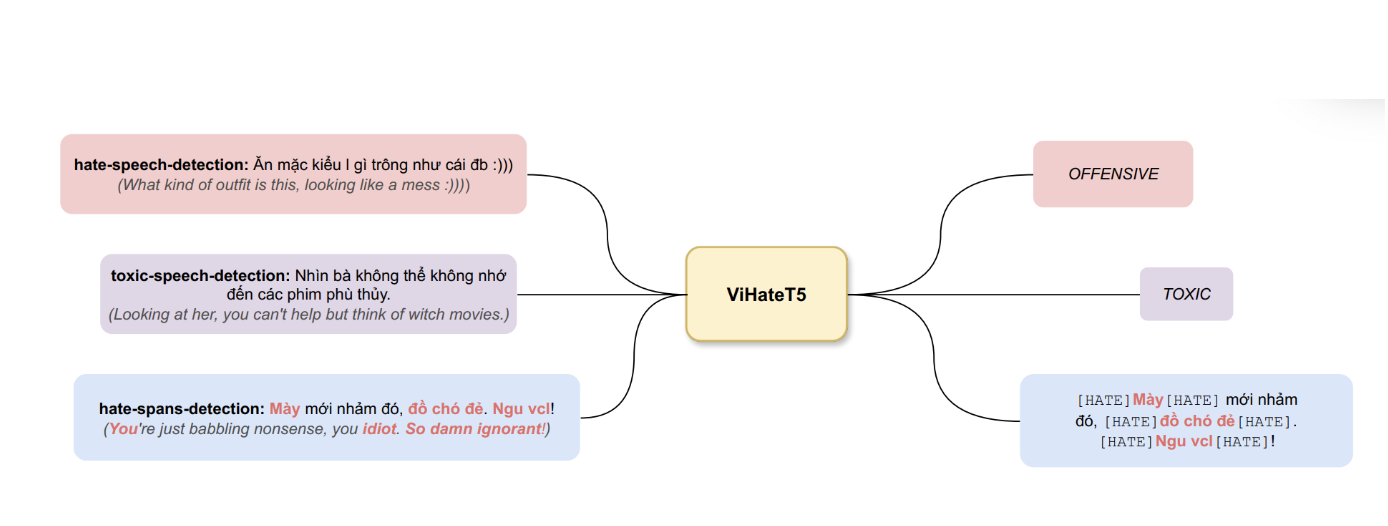
\includegraphics[width=0.82\textwidth]{Tong-quan-HSD-multitask-ViHATET5.png}
\caption{Unified Vietnamese HSD pipeline. The model receives a task prefix and generates either a label or span-marked text.}
\label{fig:pipeline}
\end{figure*}

Figure \ref{fig:pipeline} summarizes the overall text-to-text design. The same encoder-decoder backbone is reused for multiple HSD tasks, while the task prefix controls whether the decoder should generate a sentence-level label or a span-marked output. This figure motivates the later methodological choices: VOZ-HSD is used for domain adaptation, and ViHSD, ViCTSD, and ViHOS are unified during multi-task fine-tuning.

\subsection{Auto-labeling}
Auto-labeling is necessary because VOZ-HSD is large and cannot be manually annotated within the project. We convert ViHSD into a binary setting for selecting the labeling model: CLEAN remains non-hate, while OFFENSIVE and HATE are merged into a harmful class. Several BERT-style models are fine-tuned and evaluated. ViSoBERT is selected because it achieves the strongest macro score and matches the social-media domain.

\begin{figure*}[!t]
\centering
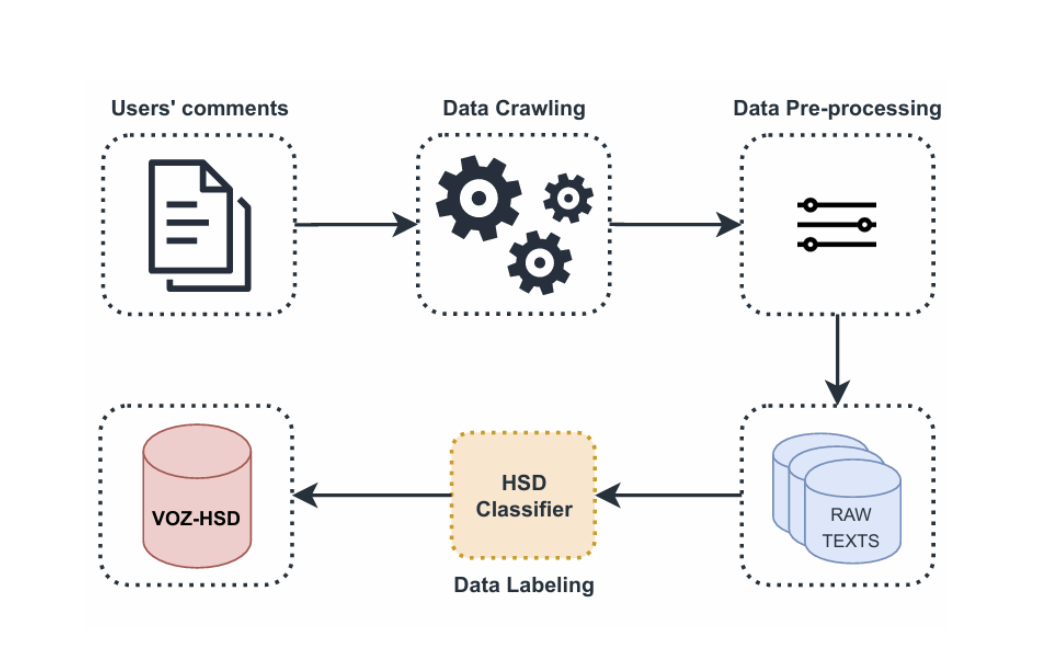
\includegraphics[width=0.82\textwidth]{So-do-quy-trinh-gan-nhan-du-lieu-VOZ-HSD.png}
\caption{VOZ-HSD collection and automatic labeling pipeline. The raw VOZ comments are processed, automatically labeled with the selected HSD classifier, and then sampled into pre-training subsets.}
\label{fig:voz_labeling_pipeline}
\end{figure*}

Figure \ref{fig:voz_labeling_pipeline} describes the bridge between raw VOZ comments and the final domain pre-training corpus. The process starts with the crawled VOZ corpus, which contains informal user discussions but does not provide reliable HSD labels for every comment. The team then prepares a binary HSD classifier by merging OFFENSIVE and HATE into one harmful class on ViHSD. After comparing BERT-style candidates, the strongest classifier is used to label the full VOZ-HSD corpus. The resulting labels allow the construction of hate-only, balanced, and full-distribution pre-training splits.

This step is crucial because it turns a large unlabeled forum corpus into a usable domain-adaptation resource. Without auto-labeling, the project would have to rely only on the much smaller downstream datasets. With auto-labeling, the model can learn from millions of informal comments before supervised fine-tuning.

\begin{table}[!t]
\centering
\caption{Auto-labeling model selection on binary ViHSD.}
\label{tab:autolabel}
\resizebox{\columnwidth}{!}{%
\begin{tabular}{lccc}
\toprule
\textbf{Model} & \textbf{Accuracy} & \textbf{Weighted-F1} & \textbf{Macro-F1} \\
\midrule
mBERT & 0.9142 & 0.9081 & 0.7604 \\
XLM-RoBERTa & 0.9197 & 0.9144 & 0.7798 \\
PhoBERT & 0.9238 & 0.9192 & 0.7947 \\
PhoBERT v2 & 0.9247 & 0.9202 & 0.7981 \\
viBERT & 0.9201 & 0.9148 & 0.7833 \\
ViSoBERT & \textbf{0.9296} & \textbf{0.8051} & \textbf{0.8128} \\
\bottomrule
\end{tabular}}
\end{table}

Although Table \ref{tab:autolabel} reports high accuracy, accuracy alone is not sufficient because harmful comments are rare. The macro score is more informative for selecting an auto-labeling model. ViSoBERT's advantage supports the hypothesis that social-media pre-training is useful for VOZ-style language.

\subsection{Domain Pre-training}
The domain pre-training stage starts from ViT5-base and continues training on VOZ-HSD with span corruption. Given an input sequence, the collator masks approximately 15\% of tokens, groups them into contiguous spans, replaces each span with a sentinel token such as \texttt{<extra\_id\_0>}, and trains the decoder to reconstruct the missing spans.

\begin{lstlisting}[style=code,caption={Simplified span corruption objective.},label={lst:span}]
Original: "May ngu qua, cho de. Im mieng di!"
Input:    "May <extra_id_0> do <extra_id_1> di!"
Target:   "<extra_id_0> ngu qua, <extra_id_1> cho de. Im mieng"
\end{lstlisting}

This objective is self-supervised. It does not teach the model to output HATE or CLEAN directly. Instead, it adapts the language model to Vietnamese forum discourse. This is essential because harmful language is often expressed through colloquial words, abbreviations, and implicit context.

\subsubsection{Span Corruption Algorithm}
For a sequence $x$ with $n$ tokens, the collator computes the number of noise tokens as $\lfloor 0.15n \rfloor$. These noise tokens are distributed into spans rather than isolated masks. Each span is replaced by a unique sentinel identifier. The target sequence is the concatenation of sentinel identifiers and the original masked spans. This differs from BERT-style masked language modeling because the decoder must generate the missing spans in order.

\begin{table}[!t]
\centering
\caption{Main functions involved in span corruption.}
\label{tab:spancode}
\resizebox{\columnwidth}{!}{%
\begin{tabular}{ll}
\toprule
\textbf{Function} & \textbf{Role} \\
\midrule
\texttt{random\_spans\_noise\_mask()} & Generate a boolean mask for noise spans \\
\texttt{create\_sentinel\_ids()} & Assign \texttt{<extra\_id>} tokens to spans \\
\texttt{filter\_input\_ids()} & Separate encoder input and decoder target \\
\texttt{compute\_t5\_input\_and\_target\_lengths()} & Preserve efficient padding lengths \\
\bottomrule
\end{tabular}}
\end{table}

Table \ref{tab:spancode} connects the mathematical objective with the actual code. This matters because span corruption is easy to describe abstractly but easy to implement incorrectly. If sentinel identifiers are not assigned consistently, the model receives invalid source-target pairs.

\subsection{Multi-task Fine-tuning}
After pre-training, all downstream datasets are converted into source-target pairs. Each source begins with a task prefix. The decoder learns to generate the corresponding label or span-marked text. Table \ref{tab:prefix} shows the unified format.

\begin{table}[!t]
\centering
\caption{Task prefix format and expected outputs.}
\label{tab:prefix}
\resizebox{\columnwidth}{!}{%
\begin{tabular}{lll}
\toprule
\textbf{Task} & \textbf{Input Prefix} & \textbf{Output} \\
\midrule
ViHSD & \texttt{hate-speech-detection: \{text\}} & CLEAN/OFFENSIVE/HATE \\
ViCTSD & \texttt{toxic-speech-detection: \{text\}} & NONE/TOXIC \\
ViHOS & \texttt{hate-spans-detection: \{text\}} & Text with [HATE] tags \\
\bottomrule
\end{tabular}}
\end{table}

The three datasets are concatenated and shuffled. This exposes the model to multiple tasks within one training run. The main advantage is architectural simplicity: one model handles classification and span marking. The trade-off is slower inference compared with encoder-only classifiers because the T5 decoder must generate text.

\subsubsection{ViHOS Post-processing}
ViHOS requires additional post-processing because the model generates text rather than direct span indices. The generated output is parsed to identify predicted span strings. The system then searches for these substrings in the original input and converts them into character-level or token-level spans. If a generated phrase cannot be found exactly, it may be counted as an error even when the phrase is semantically close.

\subsection{Improvements}
\subsubsection{Focal Loss}
Focal Loss modifies cross-entropy by down-weighting easy examples:
\begin{equation}
\mathcal{L}_{focal} = -\alpha_t (1-p_t)^\gamma \log(p_t),
\end{equation}
where $p_t$ is the probability assigned to the correct class, $\gamma$ is the focusing parameter, and $\alpha_t$ is the class-dependent weight. We use $\gamma=2$ in the experiment. The objective is useful for imbalanced datasets because easy CLEAN examples should not dominate the gradient.

\subsubsection{EDA Augmentation}
EDA augmentation is implemented in \texttt{src/augment.py}. It includes synonym replacement, random insertion, random swap, and random deletion. In our setting, it is applied to ViHSD and ViCTSD, but not to ViHOS. The reason is practical: ViHOS annotations depend on span positions, and token-level changes may invalidate the gold span boundaries.

\subsubsection{Back-translation}
Back-translation is used as an external augmentation step. Minority-class Vietnamese samples are translated into English and then translated back into Vietnamese. Samples are kept only if semantic similarity remains high. This method can create natural paraphrases, but it may remove teencode, slang, or implicit hate through translation.

\subsubsection{Ensemble}
We test majority voting and weighted ensemble. Majority voting treats every model equally:
\begin{equation}
\hat{y}=\arg\max_c \sum_{m=1}^{M} \mathbf{1}[\hat{y}_m=c].
\end{equation}
Weighted voting assigns greater influence to stronger models:
\begin{equation}
\hat{y}=\arg\max_c \sum_{m=1}^{M} w_m \mathbf{1}[\hat{y}_m=c].
\end{equation}
In our experiment, weighted ensemble matches the strongest component but does not clearly exceed it. This is an important negative result: ensemble methods help only when component models are both strong and error-complementary.

\section{Test Case Analysis}
This section analyzes representative examples from the benchmark datasets and shows how the same raw input is represented differently for BERT-based baselines and T5-based models. This comparison is important because performance differences do not come only from model architecture; they also come from the way each architecture receives supervision. BERT-based models normally receive the original sentence and learn a numeric class target. ViHateT5 receives a textual instruction prefix and learns to generate a textual answer. For span detection, the difference is even larger: BERT-style tagging uses token-level labels, while T5-style generation produces a marked sentence with \texttt{[HATE]} tokens.

\begin{table*}[!t]
\centering
\caption{Representative benchmark examples and their preprocessed representations for BERT-based baselines and T5-based models. Vietnamese examples are shown in ASCII-normalized form for LaTeX compatibility.}
\label{tab:testcase_examples}
\scriptsize
\begin{tabularx}{\textwidth}{p{0.07\textwidth}p{0.23\textwidth}p{0.08\textwidth}p{0.13\textwidth}p{0.07\textwidth}p{0.25\textwidth}p{0.10\textwidth}}
\toprule
\textbf{Dataset} & \textbf{Input Example} & \textbf{Gold Output} & \textbf{BERT Source} & \textbf{BERT Target} & \textbf{T5 Source} & \textbf{T5 Target} \\
\midrule
ViHSD &
Tu ly thuyet den thuc hanh la ca 1 cau chuyen dai. \newline
\emph{Translation: From theory to practice is a long story.} &
CLEAN &
Original sentence &
0 &
\texttt{\seqsplit{hate-speech-detection:}} Tu ly thuyet den thuc hanh la ca 1 cau chuyen dai. &
CLEAN \\
\cmidrule(lr){2-7}
ViHSD &
Giong nhau nhu 2 giot nuoc. Ma moi cai la 1 giot nuoc mat voi 1 giot nuoc s\#t thoi a. \newline
\emph{Translation: Similar as two drops of water, but one is a teardrop and the other is a drop of waste.} &
OFFENSIVE &
Original sentence &
1 &
\texttt{\seqsplit{hate-speech-detection:}} Giong nhau nhu 2 giot nuoc... &
OFFENSIVE \\
\cmidrule(lr){2-7}
ViHSD &
Im me di thang mat lon. \newline
\emph{Translation: Shut up, you big-faced idiot.} &
HATE &
Original sentence &
2 &
\texttt{\seqsplit{hate-speech-detection:}} Im me di thang mat lon. &
HATE \\
\midrule
ViCTSD &
Mot thoi de nho, bao ky niem gan lien voi nhung ca khuc cua anh. \newline
\emph{Translation: A time to remember, with many memories attached to his songs.} &
NONE &
Original sentence &
0 &
\texttt{\seqsplit{toxic-speech-detection:}} Mot thoi de nho... &
NONE \\
\cmidrule(lr){2-7}
ViCTSD &
Nghe xong mau dien trong nguoi noi len, muon danh cho thang cha mot tran qua. \newline
\emph{Translation: After listening, rage surged through my veins; I feel like giving that guy a beating.} &
TOXIC &
Original sentence &
1 &
\texttt{\seqsplit{toxic-speech-detection:}} Nghe xong mau dien... &
TOXIC \\
\midrule
ViHOS &
Hanh dien ve ng thay co tam nhat cua nam. \newline
\emph{Translation: Proud of the most dedicated teacher of the year.} &
No span &
Tokenized sentence &
All O tags &
\texttt{\seqsplit{hate-spans-detection:}} Hanh dien ve ng thay... &
Original text without \texttt{[HATE]} markers \\
\cmidrule(lr){2-7}
ViHOS &
Chuong trinh ln gi vay? :D \newline
\emph{Translation: What is this bad program?} &
Span around ``ln'' &
Tokenized sentence &
BIO/IOB tags around toxic token &
\texttt{\seqsplit{hate-spans-detection:}} Chuong trinh ln gi vay? &
Chuong trinh \texttt{[HATE]}ln\texttt{[HATE]} gi vay? \\
\cmidrule(lr){2-7}
ViHOS &
t deo hieu no cuoi cl me gi nua. \newline
\emph{Translation: I do not understand what the hell he is laughing at.} &
Multiple toxic spans &
Tokenized sentence &
BIO/IOB tags for each toxic span &
\texttt{\seqsplit{hate-spans-detection:}} t deo hieu no cuoi cl me gi nua. &
t \texttt{[HATE]}deo\texttt{[HATE]} hieu no cuoi \texttt{[HATE]}cl me\texttt{[HATE]} gi nua \\
\bottomrule
\end{tabularx}
\end{table*}

Table \ref{tab:testcase_examples} highlights the main preprocessing difference between the two model families. For BERT-based baselines, the source is usually just the original sentence. The target is a numeric ID: 0, 1, or 2 for ViHSD; 0 or 1 for ViCTSD; and a sequence of BIO/IOB-style token tags for ViHOS. This is compact and efficient. A BERT classifier only needs to map the final representation to a small set of labels. However, this compactness also means that each task requires a different output head or a different decoding rule. Sentence classification, binary toxicity detection, and span tagging are not naturally represented in one shared output space.

The T5-based representation is more verbose but more uniform. Every input begins with a natural-language-like task prefix. For ViHSD, the prefix is \texttt{hate-speech-detection:}; for ViCTSD, it is \texttt{toxic-speech-detection:}; and for ViHOS, it is \texttt{hate-spans-detection:}. The output is always text. In the first ViHSD example, the sentence is benign and the decoder is trained to generate \texttt{CLEAN}. In the second and third ViHSD examples, the decoder generates \texttt{OFFENSIVE} or \texttt{HATE}. The supervision is therefore expressed in the same language-generation framework, even though the label set changes.

The ViCTSD examples show why task prefixes are useful. A sentence can be toxic without belonging to the same label system as ViHSD. In a BERT pipeline, ViCTSD would require a separate binary classifier or at least a different classification head. In the T5 pipeline, the same model can be reused by changing the prefix and the target vocabulary. This is the main engineering advantage of ViHateT5: the system routes tasks through text instructions instead of separate model heads. The decoder learns that the toxic-speech prefix expects \texttt{NONE} or \texttt{TOXIC}, while the hate-speech prefix expects \texttt{CLEAN}, \texttt{OFFENSIVE}, or \texttt{HATE}.

The ViHOS examples show the most important difference. For BERT-based models, span detection is usually encoded as token classification. Each token receives a tag such as O, B-T, or I-T. This is precise but fragile: the tokenization scheme must align perfectly with the gold spans. If preprocessing changes token boundaries, the labels can shift. For T5-based models, the target is the original sentence with \texttt{[HATE]} markers inserted around toxic spans. This makes the task look like text editing rather than token classification. The model does not output numeric positions directly; it generates a marked sentence that is later post-processed.

This representation has both strengths and weaknesses. The strength is flexibility. T5 can handle label generation and span marking with one architecture. It can also express multiple toxic spans in one output sequence, as shown in the final ViHOS example. This is difficult to unify cleanly with ordinary classification heads. The weakness is that generation introduces new failure modes. The model may generate the right toxic phrase with slightly different spelling, may omit a marker, or may produce markers around an overlapping phrase. Such errors are not the same as ordinary classification mistakes. They are partly semantic and partly formatting-related.

The examples also clarify why macro-level scores must be interpreted carefully. A model can learn that a sentence is harmful but still confuse OFFENSIVE and HATE, as seen in the later confusion matrices. Similarly, a model can detect that a ViHOS sentence contains toxic language but fail to mark the exact span. The preprocessing format determines what the model is asked to learn. BERT is asked to classify or tag. T5 is asked to generate an answer. Therefore, comparing BERT and T5 is not only a comparison of backbones; it is also a comparison of supervision formats.

From an implementation perspective, Table \ref{tab:testcase_examples} explains why ViHateT5 is attractive for a multi-task project. The source-target abstraction allows all datasets to be concatenated and shuffled during fine-tuning. The model can see ViHSD, ViCTSD, and ViHOS examples in the same batch stream, with the prefix telling it which output format is expected. This is the reason the project emphasizes task prefixing and sequence-to-sequence fine-tuning. The price is slower inference and more post-processing, especially for span detection.

Finally, the table also explains why data augmentation must be task-aware. For ViHSD and ViCTSD, sentence-level augmentation can preserve the label if the meaning remains similar. For ViHOS, even a small word insertion or deletion can break span alignment. This is why EDA is applied to ViHSD and ViCTSD but not to ViHOS. The examples make this practical: replacing or moving words in a span-labeled sentence would require updating every span boundary or every \texttt{[HATE]} marker. Without that update, the augmented sample would become noisy supervision.

\section{Experiments}
\subsection{Implementation}
The codebase is organized around reusable modules. \texttt{src/train\_bert.py} trains encoder baselines, \texttt{src/pre\_train\_t5.py} performs domain pre-training, \texttt{src/train\_t5.py} performs multi-task fine-tuning, \texttt{src/focal\_loss.py} implements Focal Loss, \texttt{src/ensemble.py} implements ensemble inference, and \texttt{src/error\_analysis.py} generates confusion matrices and statistical summaries.

\begin{table}[!t]
\centering
\caption{Training configurations used in the reimplementation.}
\label{tab:config}
\resizebox{\columnwidth}{!}{%
\begin{tabular}{lccc}
\toprule
\textbf{Stage} & \textbf{Base Model} & \textbf{Batch} & \textbf{Epochs/LR} \\
\midrule
BERT labeling & ViSoBERT & 16 & 10 / 2e-5 \\
T5 pre-training & ViT5-base & 128--512 & 10 / 5e-3 \\
T5 fine-tuning & Pre-trained ViT5 & 32 & 4 / 2e-4 \\
Focal Loss & ViT5-base & 32 & task-specific / 2e-4 \\
\bottomrule
\end{tabular}}
\end{table}

\subsection{Evaluation Metrics}
We report \acc{}, \wf{}, and \mf{} where available. \mf{} is the main metric because label imbalance is severe. In ViHSD, a model can achieve high accuracy by predicting CLEAN frequently while still failing to detect OFFENSIVE and HATE. Weighted-F1 is still useful because it reflects performance under the empirical class distribution. However, it can hide minority-class collapse.

\subsection{Baselines}
The BERT baselines include multilingual and Vietnamese-specific encoders. The T5 baselines include mT5, ViT5, and ViHateT5-style variants. This setup allows us to separate three factors: multilingual versus Vietnamese specialization, encoder-only versus text-to-text architecture, and generic versus domain-specific pre-training.

\subsection{Reproducibility Protocol}
All reported results are derived from artifacts saved under \texttt{results/}. We separate raw evaluation metrics, analysis outputs, and figures. This prevents a common reporting error: copying a number from a slide without tracking its source. When a value comes from the paper rather than our reimplementation, the source column explicitly says ``Paper.''

\section{Results and Discussion}
\subsection{T5 Reimplementation Results}
Table \ref{tab:t5models} compares the main T5-family models. The balanced ViHateT5-style variant obtains the best average score among our T5 experiments. Its average \mf{} is 0.7501, slightly above ViT5-base and clearly above mT5-base.

\begin{table*}[!t]
\centering
\caption{Macro-F1 comparison of text-to-text models.}
\label{tab:t5models}
\begin{tabular}{llcccc}
\toprule
\textbf{Model} & \textbf{Source} & \textbf{ViHSD} & \textbf{ViCTSD} & \textbf{ViHOS} & \textbf{Average} \\
\midrule
ViT5-base & Ours & 0.6625 & 0.7163 & 0.8612 & 0.7467 \\
mT5-base & Ours & 0.6246 & 0.7053 & 0.8501 & 0.7267 \\
ViHateT5-style balanced & Ours & \textbf{0.6698} & \textbf{0.7189} & \textbf{0.8616} & \textbf{0.7501} \\
ViHateT5 paper full & Paper & 0.6867 & 0.7358 & 0.8644 & 0.7623 \\
\bottomrule
\end{tabular}
\end{table*}

The gap between our balanced variant and the paper's full-data setting is expected because the original paper uses substantially more pre-training data. However, our result suggests that careful data selection can recover much of the benefit at a smaller scale. The stronger result of ViT5 over mT5 also confirms the value of Vietnamese-specific pre-training.

\begin{table*}[!t]
\centering
\caption{Detailed T5 evaluation metrics from our reimplementation.}
\label{tab:t5detail}
\begin{tabular}{llccc}
\toprule
\textbf{Model} & \textbf{Dataset} & \textbf{Accuracy} & \textbf{Weighted-F1} & \textbf{Macro-F1} \\
\midrule
\multirow{3}{*}{ViT5-base}
& ViHSD & 0.8777 & 0.8787 & 0.6625 \\
& ViCTSD & 0.9080 & 0.9178 & 0.7163 \\
& ViHOS & 0.9075 & 0.9000 & 0.8612 \\
\midrule
\multirow{3}{*}{mT5-base}
& ViHSD & 0.8746 & 0.8877 & 0.6246 \\
& ViCTSD & 0.8932 & 0.9024 & 0.7053 \\
& ViHOS & 0.9075 & 0.8957 & 0.8501 \\
\midrule
\multirow{3}{*}{ViHateT5-style balanced}
& ViHSD & 0.8815 & 0.8849 & 0.6698 \\
& ViCTSD & 0.9105 & 0.9158 & 0.7189 \\
& ViHOS & 0.9081 & 0.9055 & 0.8616 \\
\bottomrule
\end{tabular}
\end{table*}

Table \ref{tab:t5detail} expands the compact \mf{} comparison. It shows that the balanced variant maintains strong accuracy and weighted scores while slightly improving macro performance. The differences are not dramatic, but they are consistent with the hypothesis that domain adaptation is more valuable than simply switching between T5-family backbones.

\subsection{Pre-training Strategy}
Table \ref{tab:pretrain} compares hate-only and balanced pre-training. Hate-only improves ViHSD, but balanced pre-training improves ViCTSD and ViHOS more strongly, yielding the best average score.

\begin{table*}[!t]
\centering
\caption{Downstream \mf{} for different pre-training strategies.}
\label{tab:pretrain}
\begin{tabular}{llcccc}
\toprule
\textbf{Model} & \textbf{Source} & \textbf{ViHSD} & \textbf{ViCTSD} & \textbf{ViHOS} & \textbf{Average} \\
\midrule
ViHateT5 & Paper (584K hate-only) & 0.6548 & 0.6134 & 0.8542 & 0.7075 \\
ViHateT5 & Ours (100K hate-only) & \textbf{0.6808} & 0.6586 & 0.8541 & 0.7312 \\
ViHateT5 & Paper (1.17M balanced) & 0.6600 & 0.6022 & 0.8577 & 0.7066 \\
ViHateT5 & Ours (200K balanced) & 0.6698 & 0.7189 & 0.8616 & \textbf{0.7501} \\
ViHateT5 & Paper (10.8M full) & 0.6867 & \textbf{0.7358} & \textbf{0.8644} & \textbf{0.7623} \\
\bottomrule
\end{tabular}
\end{table*}

The main lesson is that ``more data'' and ``better class balance'' are different factors. Full data provides broad coverage, but its label distribution is extremely skewed. Balanced data exposes the model to both harmful and non-harmful patterns. Hate-only data emphasizes harmful expressions but may remove useful negative examples needed for contrastive understanding.

\subsection{BERT Baselines}
Table \ref{tab:bert} summarizes BERT-style baselines. ViSoBERT performs very strongly, especially on ViHOS, which supports the value of social-media pre-training. However, BERT models still require different output handling for different tasks.

\begin{table*}[!t]
\centering
\caption{BERT baseline results on three downstream datasets.}
\label{tab:bert}
\begin{tabular}{llccc}
\toprule
\textbf{Model} & \textbf{Source} & \textbf{ViHSD} & \textbf{ViCTSD} & \textbf{ViHOS} \\
\midrule
BERT cased & Ours & 0.6427 & 0.6886 & 0.8832 \\
XLM-RoBERTa & Ours & 0.6544 & 0.7231 & 0.8878 \\
PhoBERT v2 & Ours & 0.6583 & 0.7304 & 0.9031 \\
PhoBERT & Ours & 0.6360 & 0.7210 & 0.8903 \\
BERT uncased & Ours & 0.6161 & 0.6569 & 0.8706 \\
DistilBERT & Ours & 0.6224 & 0.6634 & 0.8706 \\
viBERT & Ours & 0.6149 & 0.6946 & 0.8589 \\
ViSoBERT & Ours & \textbf{0.6871} & \textbf{0.7483} & \textbf{0.9230} \\
ViHateT5 & Paper & 0.6867 & 0.7358 & 0.8637 \\
\bottomrule
\end{tabular}
\end{table*}

The ViSoBERT results are notable because they show that an encoder-only model can be highly competitive when its pre-training domain matches the target data. Nevertheless, the unified T5 approach remains attractive when one system must support sentence classification and span generation simultaneously.

\subsection{Focal Loss Results}
Table \ref{tab:focal} reports the controlled Focal Loss comparison on ViHSD. Focal Loss improves \mf{} from 0.5198 to 0.7478 and improves accuracy from 0.8882 to 0.9172 in this setup. However, the OFFENSIVE score remains zero, meaning the improvement is not uniformly distributed across all labels.

\begin{table}[!t]
\centering
\caption{Cross-entropy versus Focal Loss on ViHSD.}
\label{tab:focal}
\begin{tabular}{lcc}
\toprule
\textbf{Metric} & \textbf{Cross-Entropy} & \textbf{Focal Loss} \\
\midrule
\mf{} & 0.5198 & \textbf{0.7478} \\
\acc{} & 0.8882 & \textbf{0.9172} \\
F1 CLEAN & 0.9401 & \textbf{0.9545} \\
F1 OFFENSIVE & 0.0000 & 0.0000 \\
F1 HATE & \textbf{0.6194} & 0.5411 \\
\bottomrule
\end{tabular}
\end{table}

This table is important for interpretation. Focal Loss is a useful improvement, but it is not a universal replacement for balanced pre-training. It helps ViHSD under a specific class-imbalance setting, yet the balanced checkpoint remains stronger on average across all three downstream datasets.

\subsection{Macro-F1 Comparison of Improvement Variants}
Table \ref{tab:variants} compares the Focal Loss experiment with the balanced and hate-only fine-tuning variants. The Focal Loss experiment has the highest ViHSD score, while the balanced variant has the best average score.

\begin{table}[!t]
\centering
\caption{\mf{} comparison of T5 variants.}
\label{tab:variants}
\resizebox{\columnwidth}{!}{%
\begin{tabular}{lcccc}
\toprule
\textbf{Model} & \textbf{ViHSD} & \textbf{ViCTSD} & \textbf{ViHOS} & \textbf{Avg.} \\
\midrule
\model{vit5\_focal\_loss\_exp} & \textbf{0.7478} & 0.5382 & 0.8247 & 0.7036 \\
\model{vit5\_finetune\_balanced} & 0.6698 & \textbf{0.7189} & \textbf{0.8616} & \textbf{0.7501} \\
\model{vit5\_finetune\_hate\_only} & 0.6808 & 0.6586 & 0.8541 & 0.7312 \\
\bottomrule
\end{tabular}}
\end{table}

This result resolves a potential confusion in the slide deck. Focal Loss is an improvement for a particular ViHSD experiment, but the balanced model is the better all-round model. Therefore, the correct conclusion is not ``Focal Loss is always best,'' but rather ``Focal Loss targets class imbalance, while balanced domain pre-training gives better multi-dataset robustness.''

\subsection{Ensemble Results}
Table \ref{tab:ensemble} reports ensemble results on ViHSD. Weighted ensemble matches the balanced model, while majority voting is weaker.

\begin{table}[!t]
\centering
\caption{Individual and ensemble results on ViHSD.}
\label{tab:ensemble}
\resizebox{\columnwidth}{!}{%
\begin{tabular}{lcccc}
\toprule
\textbf{Method} & \textbf{Acc.} & \textbf{\mf{}} & \textbf{F1 CLEAN} & \textbf{F1 HATE} \\
\midrule
\model{vit5\_finetune\_balanced} & 0.8046 & \textbf{0.6346} & 0.9412 & \textbf{0.7273} \\
\model{vit5\_focal\_loss\_exp} & 0.7701 & 0.5277 & 0.8909 & 0.6923 \\
\model{visobert\_labeling} & 0.7241 & 0.4775 & 0.8547 & 0.5778 \\
Weighted ensemble & \textbf{0.8046} & \textbf{0.6346} & \textbf{0.9412} & \textbf{0.7273} \\
Majority voting & 0.7701 & 0.5317 & 0.8750 & 0.7200 \\
\bottomrule
\end{tabular}}
\end{table}

The ensemble result is modest because the component models are not equally reliable and do not make sufficiently complementary errors. Majority voting treats weak and strong models equally, so weaker predictions can drag the final decision down. Weighted voting is safer, but in this experiment it mainly reproduces the best component.

\subsection{Visual Analysis}
Figures \ref{fig:modelcompare}--\ref{fig:ratio} visualize the same trends. The overall comparison highlights differences between BERT and T5 families. The T5-only chart shows the advantage of ViHateT5-style domain adaptation. The ranking and radar charts provide a compact view of model balance across tasks.

\begin{figure*}[!t]
\centering
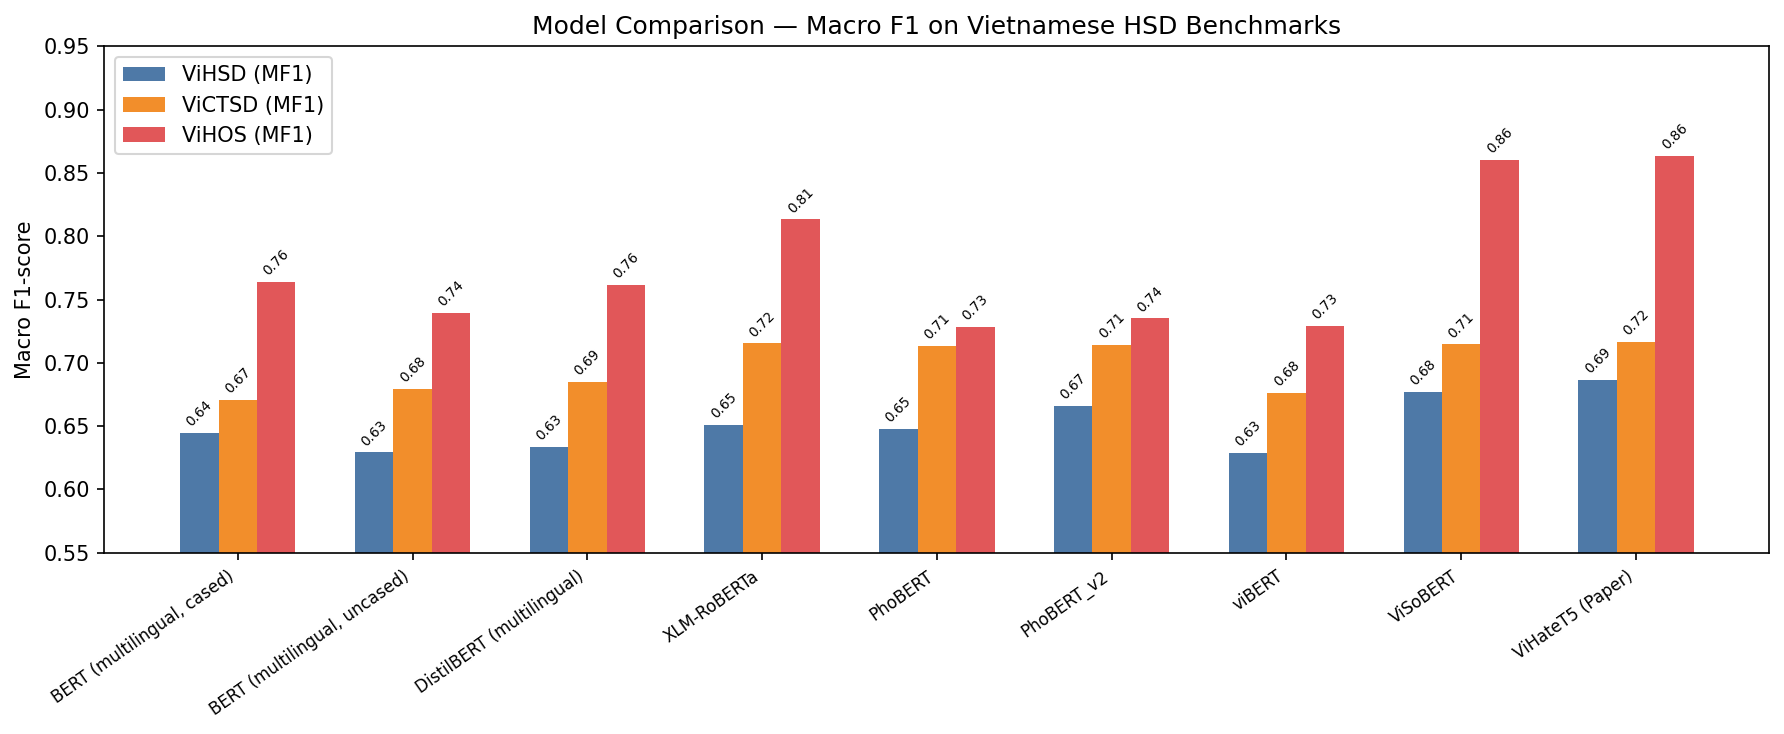
\includegraphics[width=0.88\textwidth]{model_comparison_macro_f1.png}
\caption{Macro-F1 comparison across Vietnamese HSD benchmarks.}
\label{fig:modelcompare}
\end{figure*}

\begin{figure*}[!t]
\centering
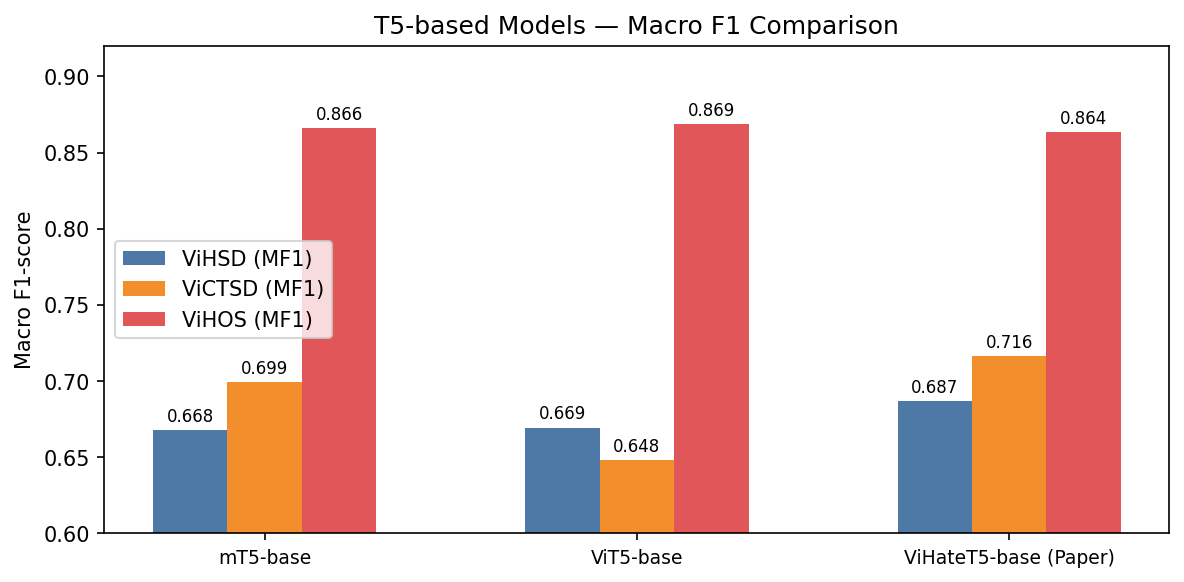
\includegraphics[width=0.82\textwidth]{t5_comparison_macro_f1.png}
\caption{Macro-F1 comparison of T5-family models.}
\label{fig:t5compare}
\end{figure*}

\begin{figure*}[!t]
\centering
\begin{subfigure}{0.48\textwidth}
\centering
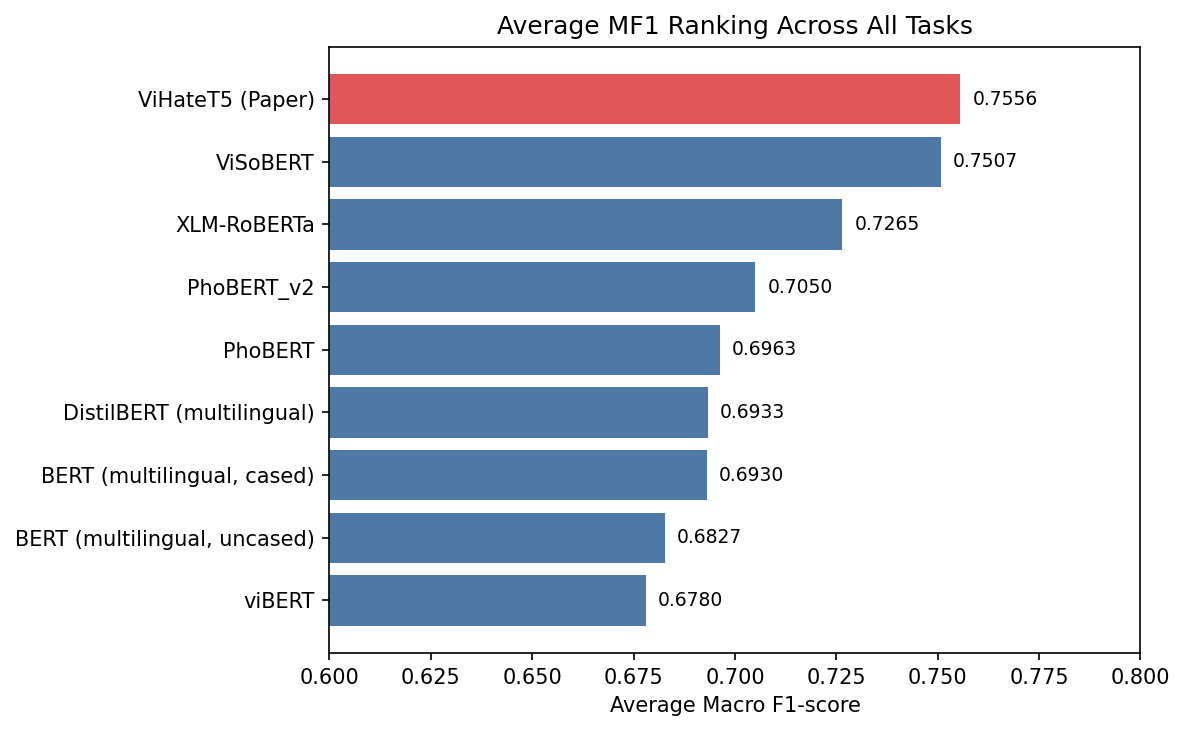
\includegraphics[width=\linewidth]{average_mf1_ranking.png}
\caption{Average \mf{} ranking.}
\end{subfigure}
\hfill
\begin{subfigure}{0.48\textwidth}
\centering
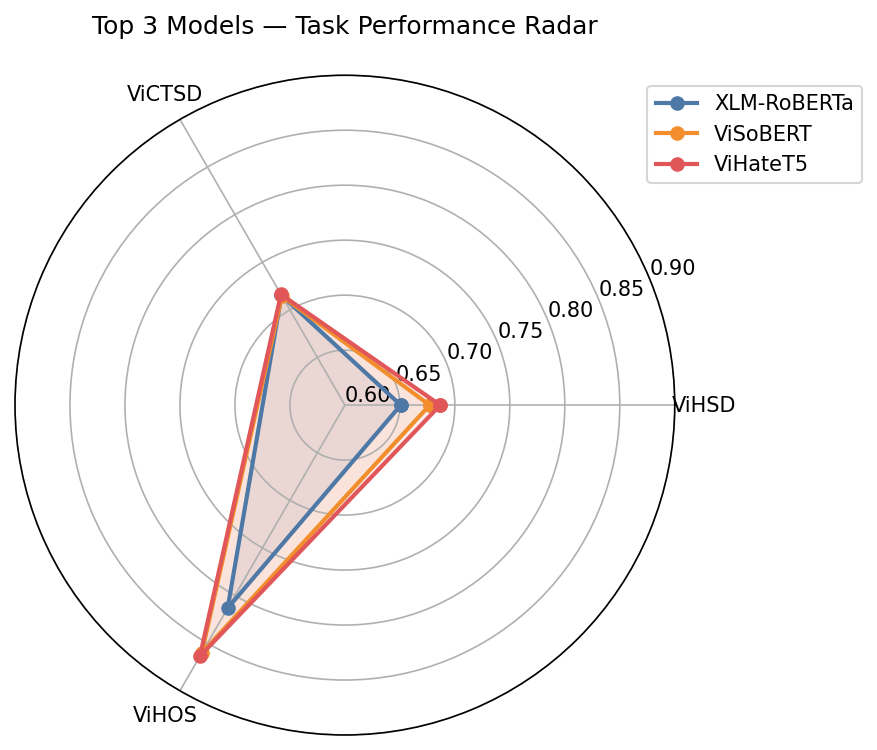
\includegraphics[width=\linewidth]{radar_top3_models.png}
\caption{Radar chart for top models.}
\end{subfigure}
\caption{Ranking and balance analysis across datasets.}
\label{fig:ranking}
\end{figure*}

\begin{figure*}[!t]
\centering
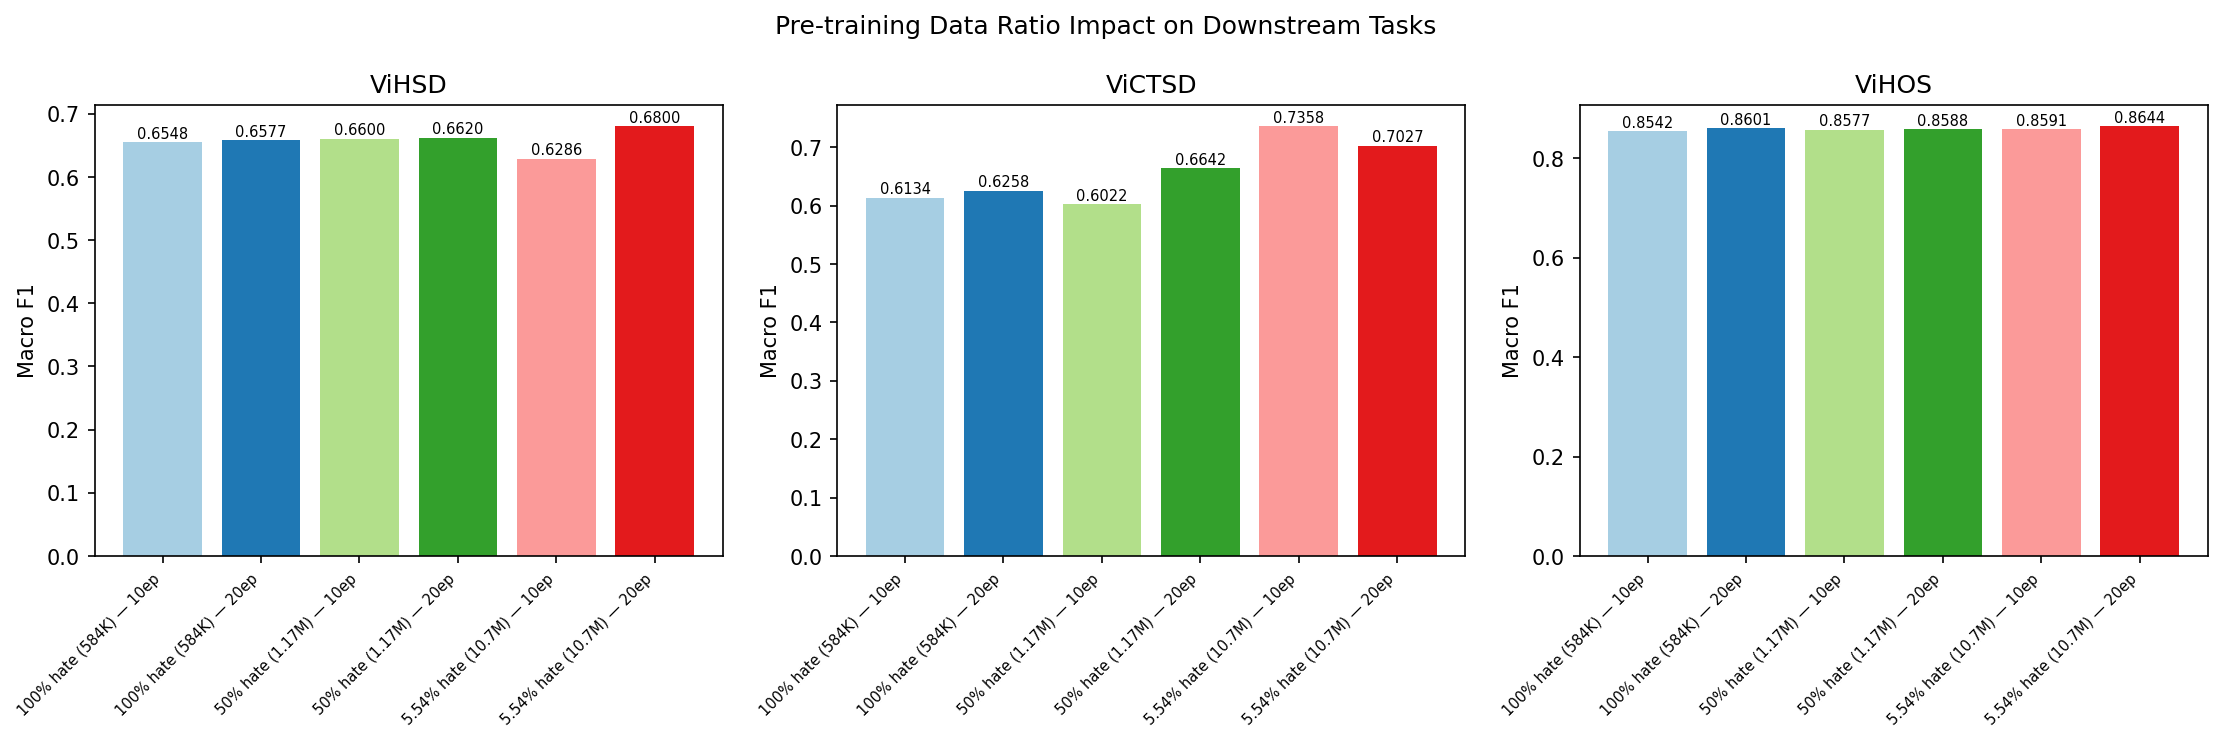
\includegraphics[width=0.82\textwidth]{pretrain_data_ratio_impact.png}
\caption{Impact of pre-training data ratio on downstream performance.}
\label{fig:ratio}
\end{figure*}

The visualizations are not used as primary evidence; the tables remain the authoritative source. Their purpose is diagnostic. A bar chart makes it easier to see whether a model is strong across all tasks or only on one benchmark. The radar chart is especially useful because the goal is multi-task robustness, not single-dataset optimization.

\section{Error Analysis}
\subsection{Per-class Behavior}
Table \ref{tab:perclass} shows per-class behavior for two important variants. The balanced model is more stable across the three classes, while the Focal Loss model improves some metrics but fails on OFFENSIVE in this split.

\begin{table}[!t]
\centering
\caption{Per-class report on ViHSD for two T5 variants.}
\label{tab:perclass}
\resizebox{\columnwidth}{!}{%
\begin{tabular}{llccc}
\toprule
\textbf{Model} & \textbf{Class} & \textbf{Precision} & \textbf{Recall} & \textbf{F1} \\
\midrule
\multirow{3}{*}{Balanced} & CLEAN & 0.8972 & 0.9600 & 0.9275 \\
& OFFENSIVE & 0.3636 & 0.1739 & 0.2353 \\
& HATE & 0.6545 & 0.7200 & 0.6857 \\
\midrule
\multirow{3}{*}{Focal Loss} & CLEAN & 0.7857 & 0.9900 & 0.8761 \\
& OFFENSIVE & 0.0000 & 0.0000 & 0.0000 \\
& HATE & 0.6383 & 0.6000 & 0.6186 \\
\bottomrule
\end{tabular}}
\end{table}

OFFENSIVE is consistently the hardest class. This is not surprising because offensive language can be rude without targeting a protected group, while hate speech often requires target-group interpretation. In Vietnamese social-media text, this boundary is blurry. Some comments are insults between individuals, some are group attacks, and some require thread context.

\subsection{Confusion Matrices and Error Distribution}
Figure \ref{fig:cm} shows confusion matrices for representative models. Most errors occur around minority classes. CLEAN is relatively easy because it dominates training data and has more stable linguistic patterns. OFFENSIVE and HATE have fewer samples and overlap semantically.

\begin{figure*}[!t]
\centering
\begin{subfigure}{0.48\textwidth}
\centering
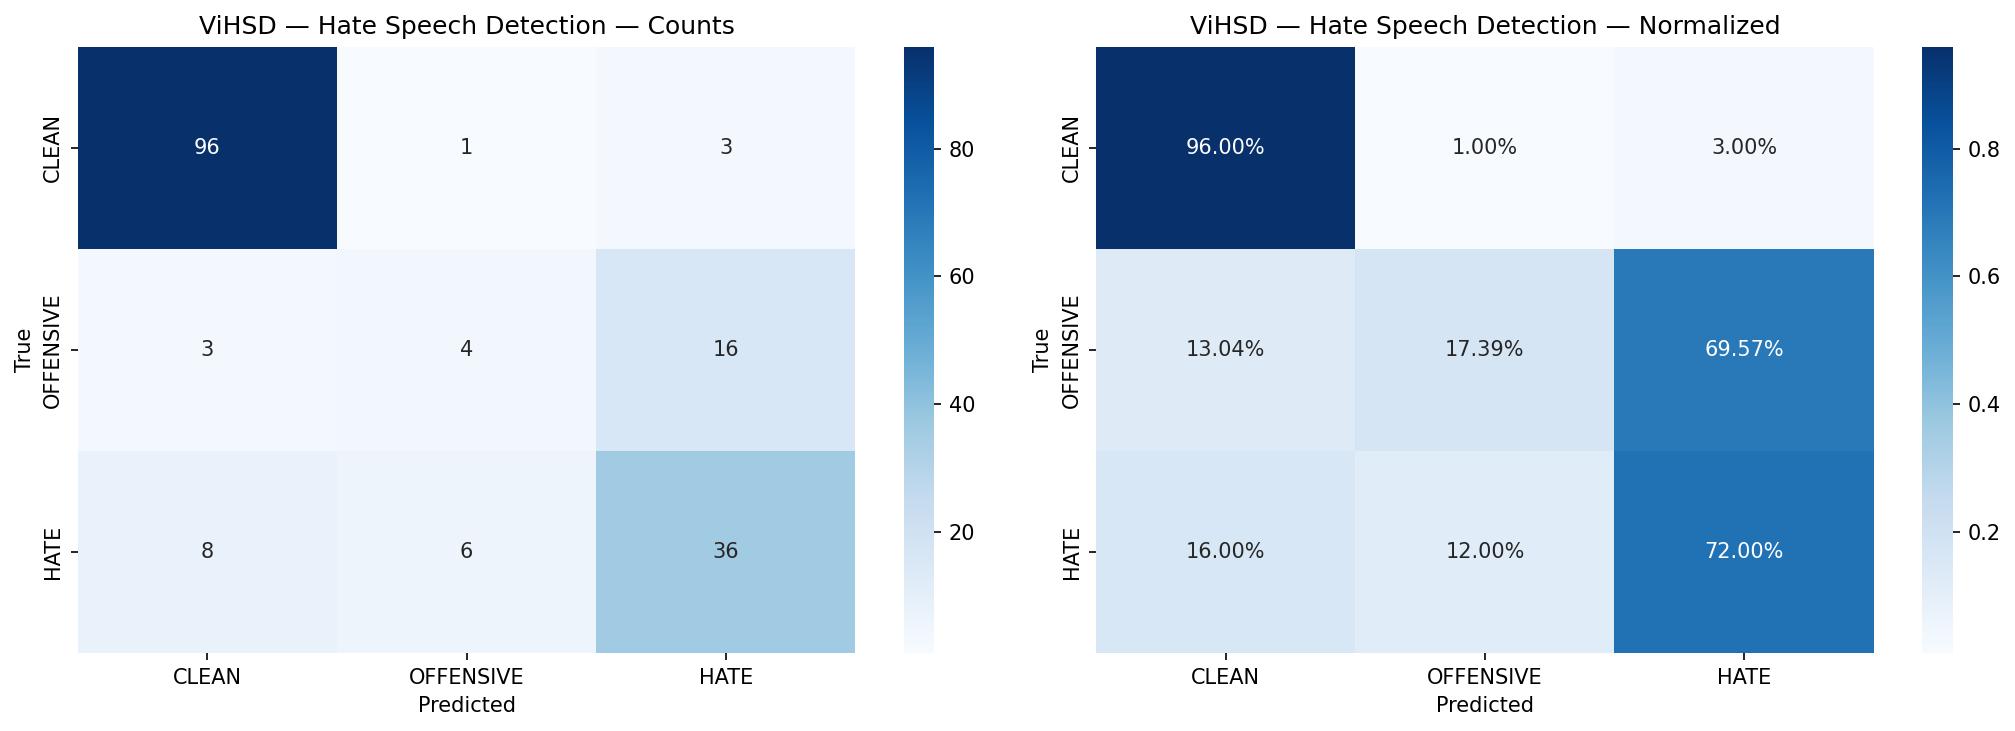
\includegraphics[width=\linewidth]{confusion_matrix_vihsd_vit5_finetune_balanced.png}
\caption{ViT5 balanced.}
\end{subfigure}
\hfill
\begin{subfigure}{0.48\textwidth}
\centering
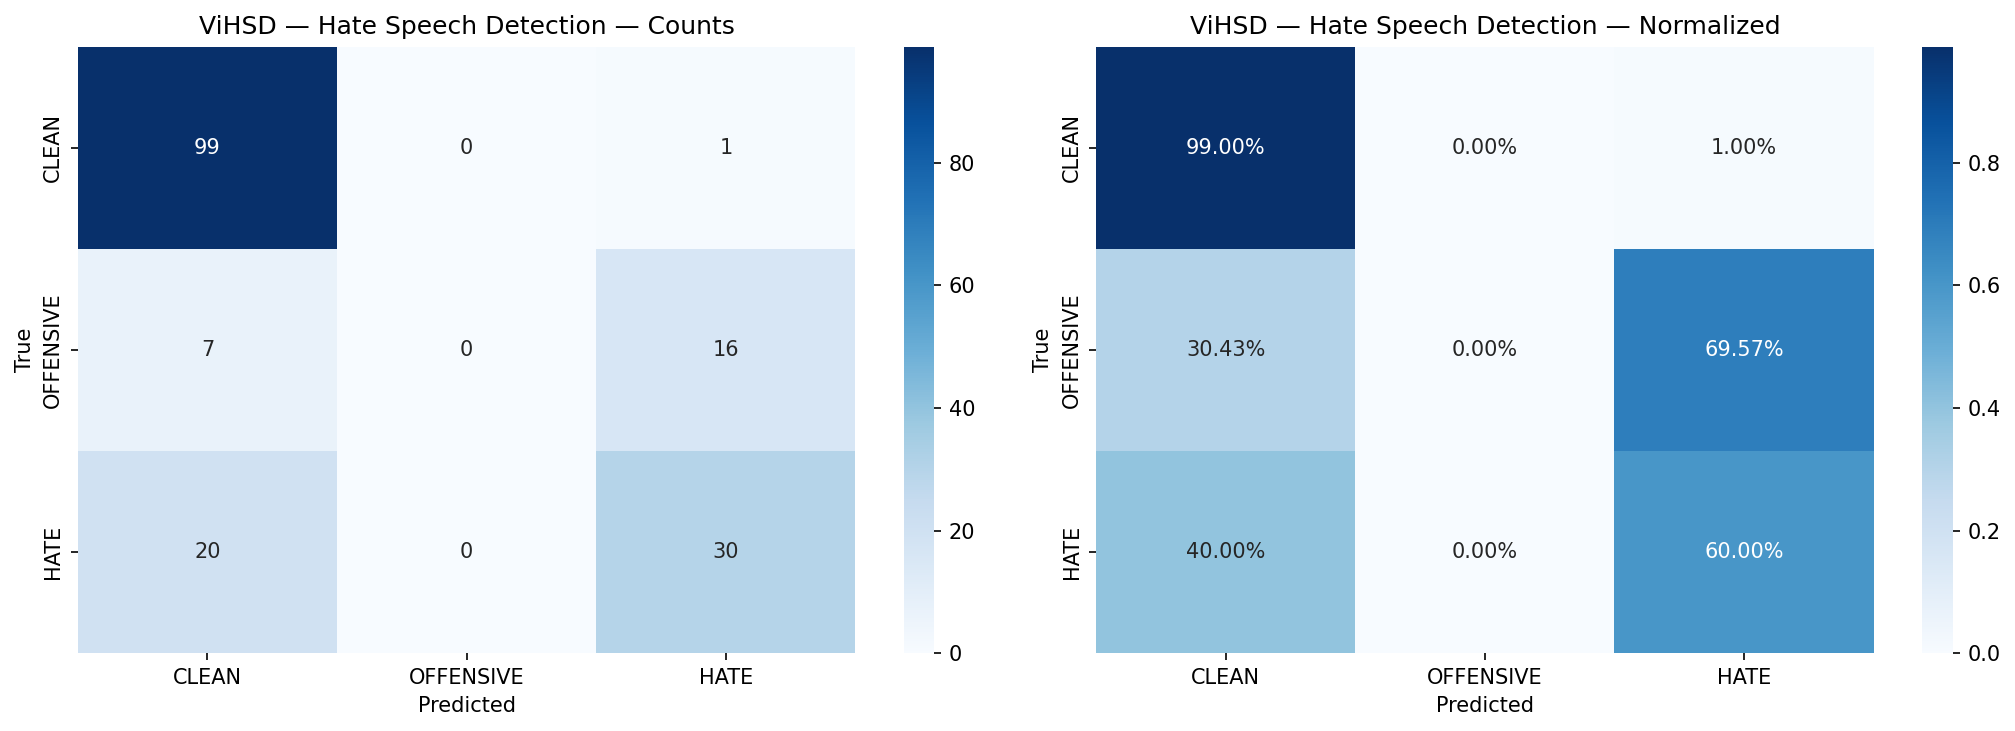
\includegraphics[width=\linewidth]{confusion_matrix_vihsd_vit5_focal_loss_exp.png}
\caption{ViT5 Focal Loss.}
\end{subfigure}
\caption{Confusion matrices on ViHSD.}
\label{fig:cm}
\end{figure*}

\begin{figure*}[!t]
\centering
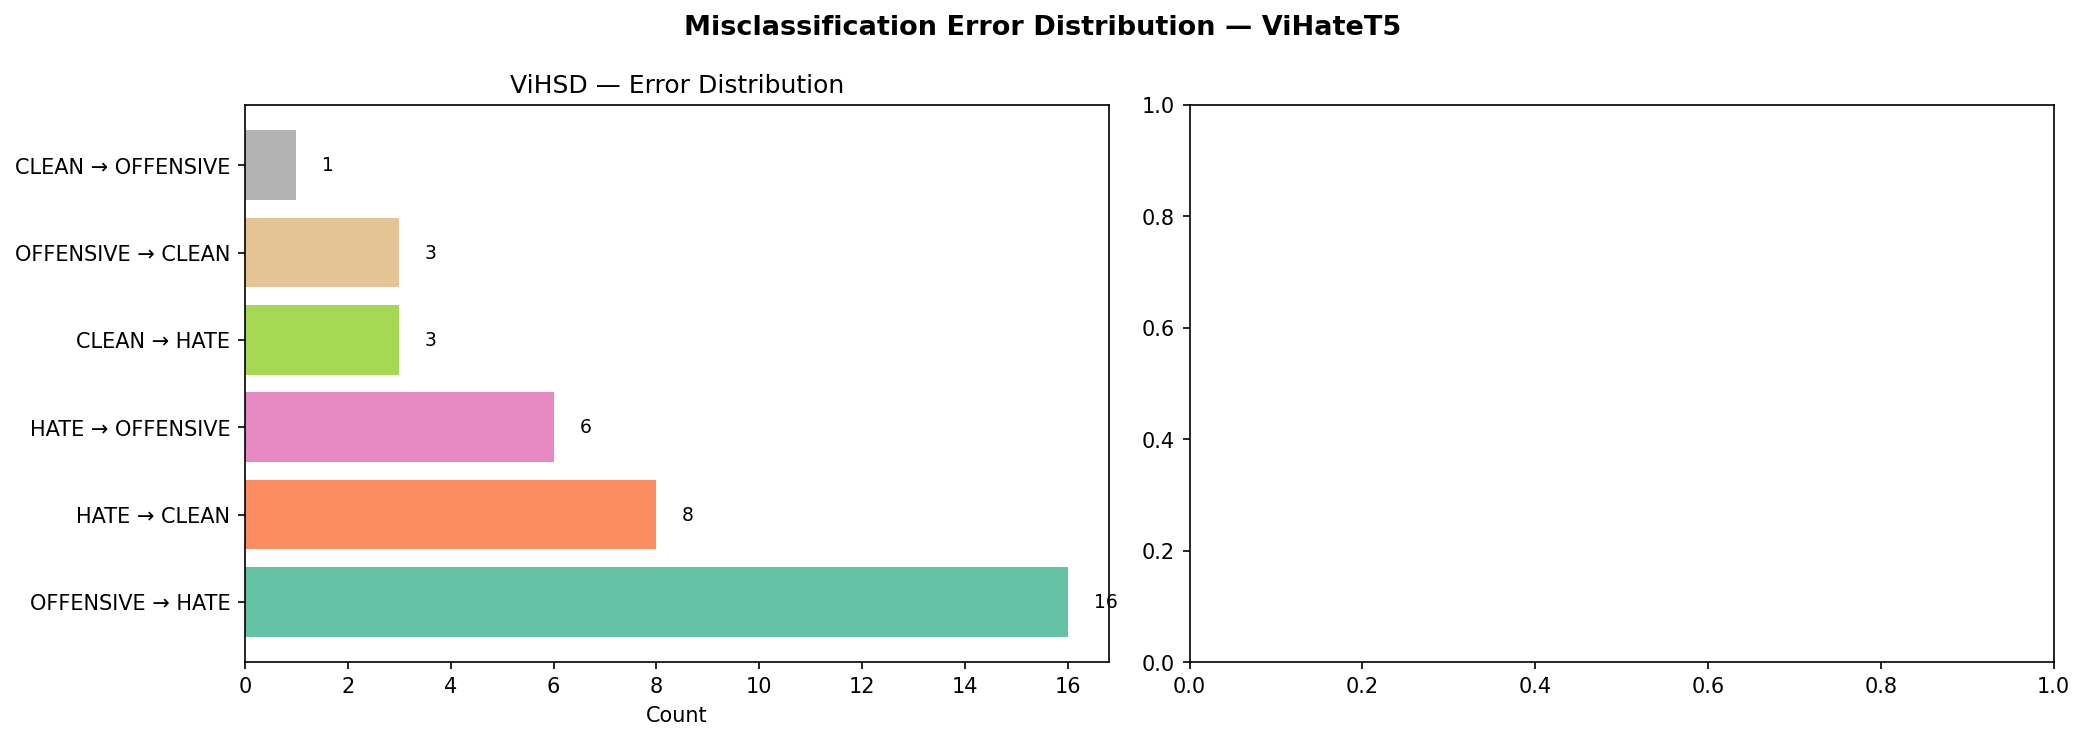
\includegraphics[width=0.82\textwidth]{error_distribution_vit5_finetune_balanced.png}
\caption{Error distribution for the balanced variant.}
\label{fig:error}
\end{figure*}

Figure \ref{fig:error} complements the confusion matrix by summarizing error types rather than only class-to-class transitions. The balanced model still makes mistakes on minority labels, but its errors are less extreme than variants that collapse one class entirely. This supports the main conclusion that balanced pre-training is not always the best on one isolated score, but it is the most stable strategy across labels and datasets.

\subsection{Qualitative Failure Categories}
The failure cases can be grouped into four categories. The first category is boundary confusion between OFFENSIVE and HATE. This occurs when a sentence contains strong insults but does not clearly target a protected group. The second category is implicit hate, where the harmful meaning is expressed indirectly. The third category is slang and teencode, where tokenization and normalization affect interpretation. The fourth category is context dependence, where a comment cannot be judged accurately without the parent comment or conversation history.

\begin{table}[!t]
\centering
\caption{Representative qualitative failure categories.}
\label{tab:failures}
\resizebox{\columnwidth}{!}{%
\begin{tabular}{p{0.27\columnwidth}p{0.33\columnwidth}p{0.31\columnwidth}}
\toprule
\textbf{Category} & \textbf{Typical Cause} & \textbf{Model Risk} \\
\midrule
OFFENSIVE/HATE boundary & Insult words without clear group target & Over-predict HATE or collapse to OFFENSIVE \\
Implicit hate & Harmful intent is indirect or sarcastic & False negative \\
Teencode/slang & Informal spelling and abbreviations & Tokenization mismatch \\
Context dependence & Meaning depends on previous messages & Incorrect sentence-level label \\
\bottomrule
\end{tabular}}
\end{table}

This qualitative analysis explains why augmentation must be used carefully. Back-translation can create paraphrases, but it can also remove slang or soften implicit hate. EDA can increase minority-class diversity, but random deletion or swapping can change the intensity of an insult.

\subsection{Statistical Significance}
Table \ref{tab:mcnemar} reports McNemar tests against the balanced baseline. The test checks whether two models differ significantly on paired predictions. ViHateT5 reimplementation and ViSoBERT differ significantly from the balanced variant, while other ViT5 variants do not show a reliable difference in this test.

\begin{table}[!t]
\centering
\caption{McNemar test on ViHSD against \model{vit5\_finetune\_balanced}.}
\label{tab:mcnemar}
\resizebox{\columnwidth}{!}{%
\begin{tabular}{lccc}
\toprule
\textbf{Comparison Model} & $\chi^2$ & \textbf{p-value} & \textbf{Significant} \\
\midrule
\model{vihatet5\_reimpl} & 63.3772 & $<0.001$ & Yes \\
\model{visobert\_labeling} & 9.4464 & 0.0021 & Yes \\
\model{vit5\_finetune\_hate\_only} & 0.0833 & 0.7728 & No \\
\model{vit5\_finetune\_multi} & 0.0556 & 0.8137 & No \\
\model{vit5\_focal\_loss\_exp} & 1.8947 & 0.1687 & No \\
\bottomrule
\end{tabular}}
\end{table}

Statistical testing prevents overinterpreting small score differences. A variant may have a slightly higher score but still fail to produce a statistically reliable difference on paired examples. This is particularly important for small test subsets and imbalanced labels.

\section{Demo System}
The demo system provides an interface for testing Vietnamese HSD predictions. A user enters a Vietnamese sentence, the web application sends the text to the inference backend, and the backend returns the predicted label. The demo is not intended to replace human moderation. Instead, it demonstrates how a trained model can support triage and prioritization.

\begin{figure*}[!t]
\centering
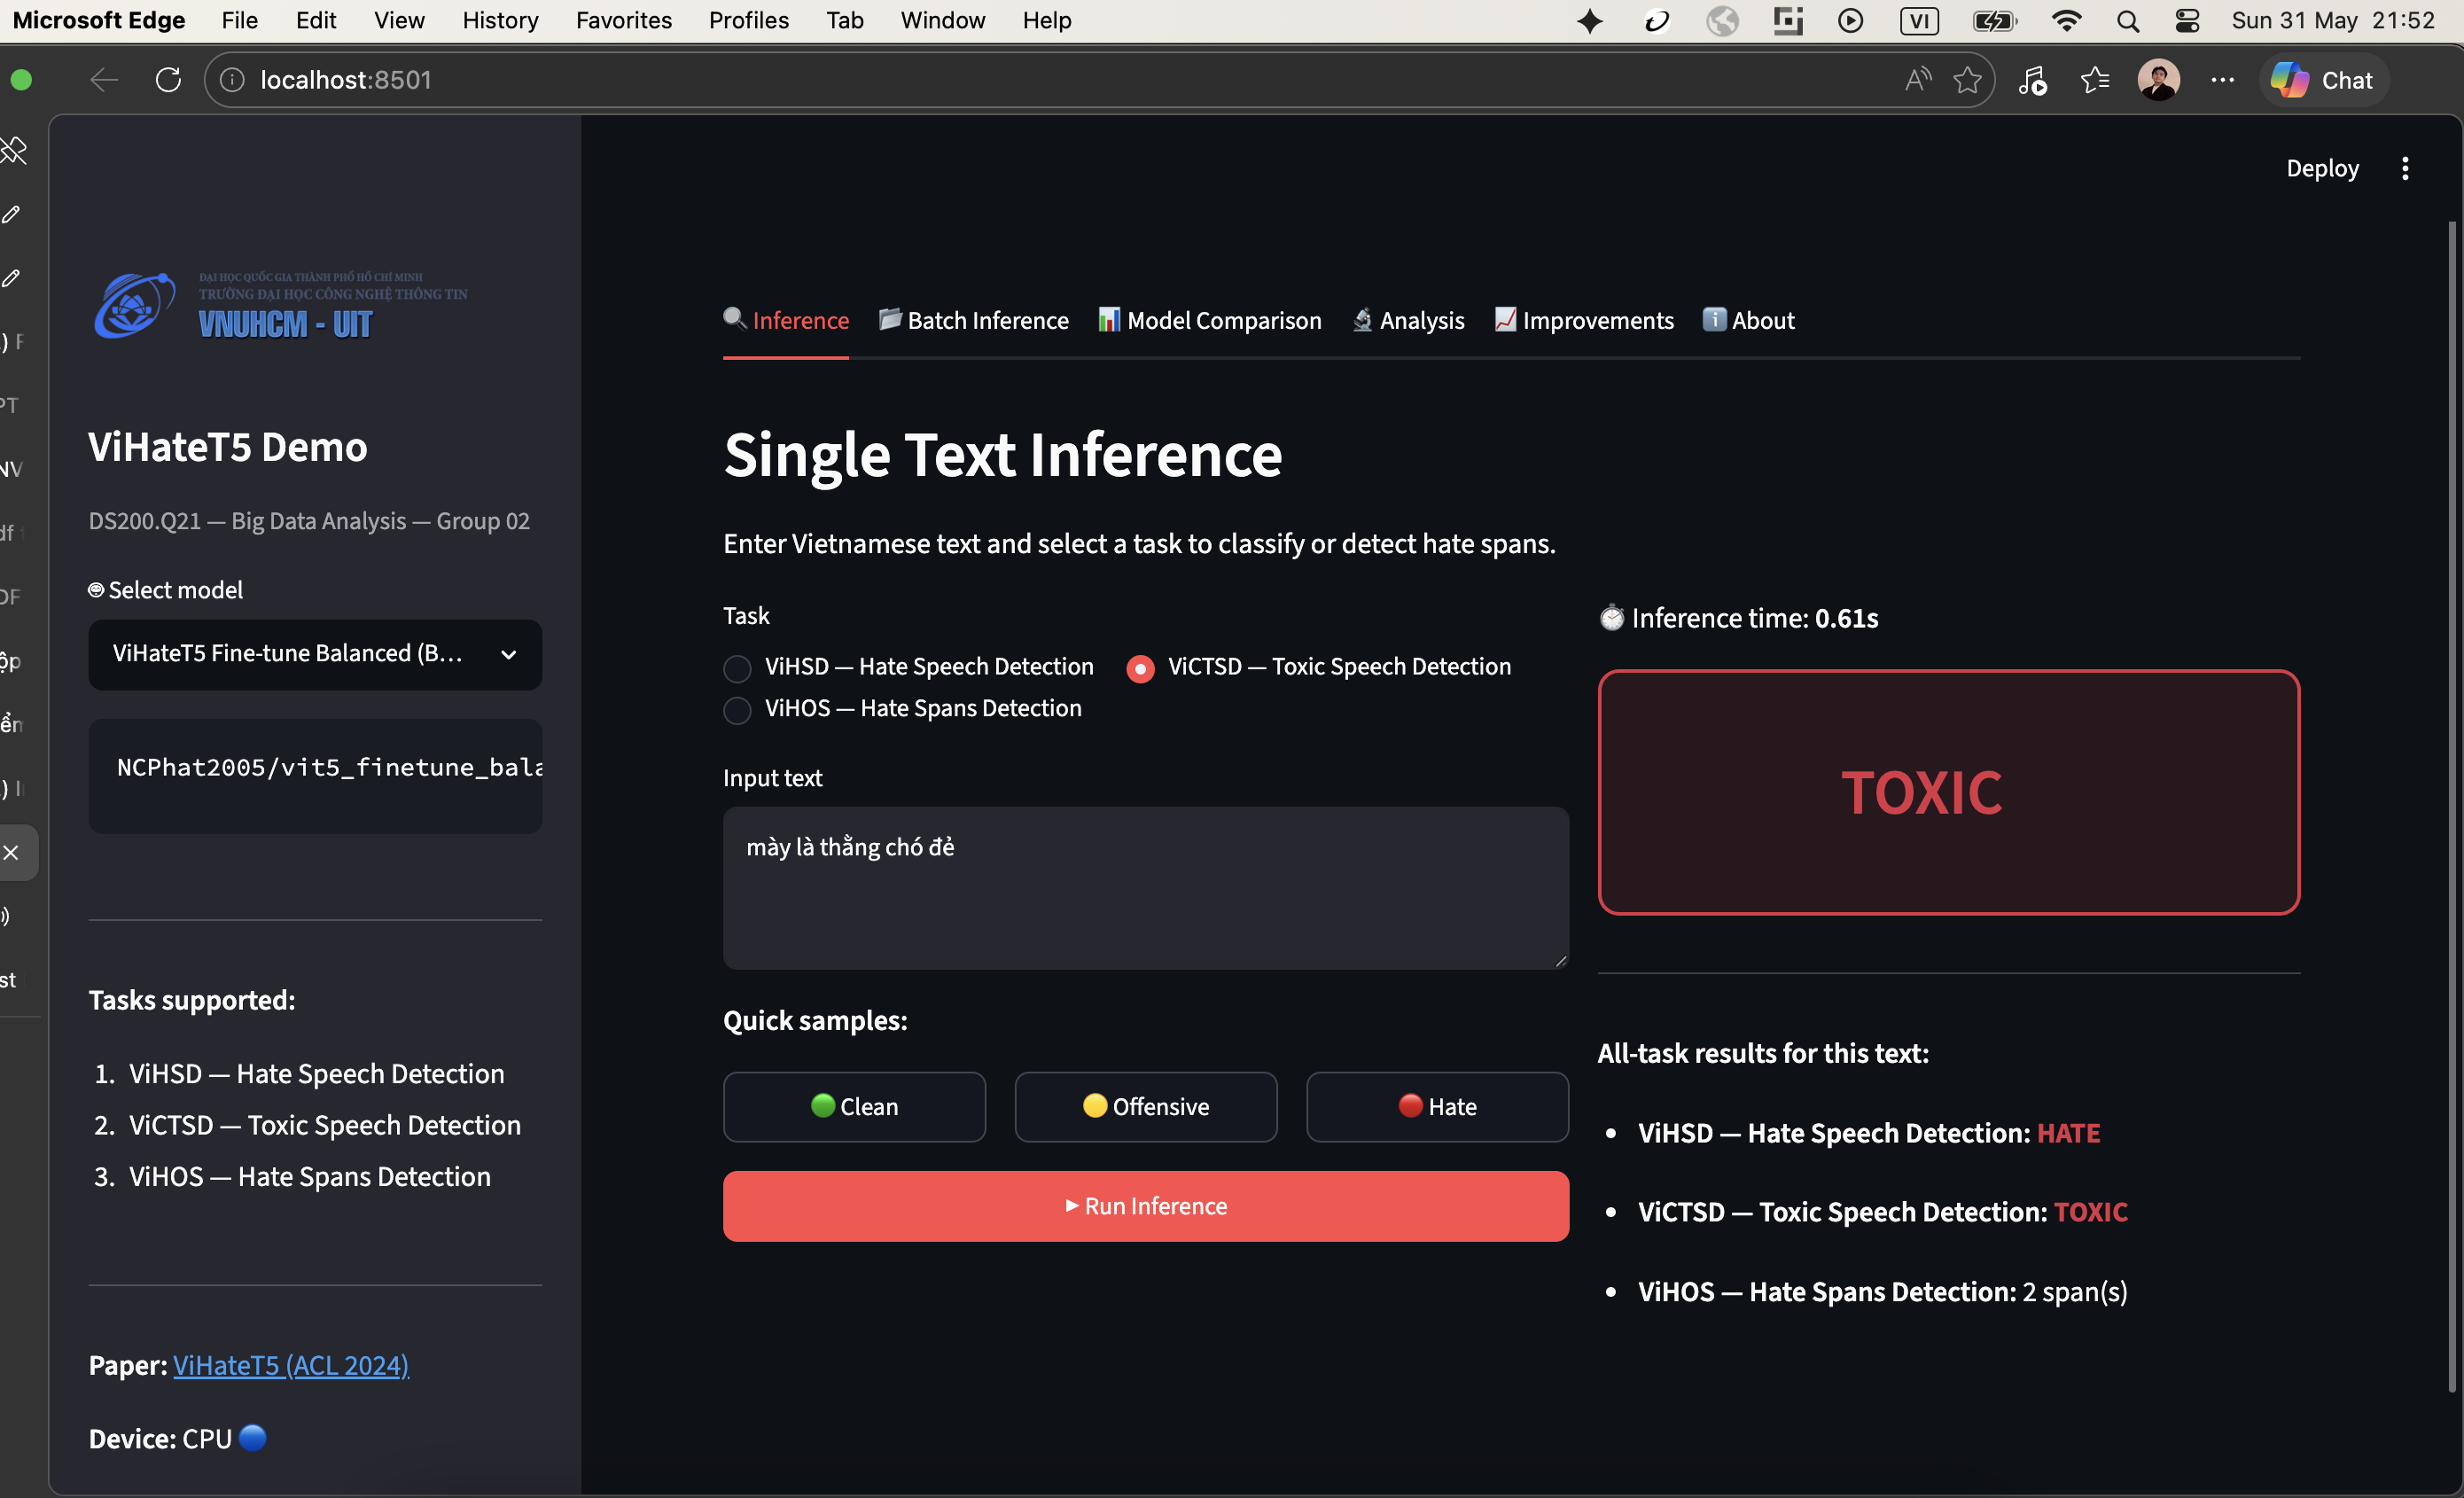
\includegraphics[width=0.82\textwidth]{demo_webapp.png}
\caption{Interactive web demo for Vietnamese hate speech detection.}
\label{fig:demo}
\end{figure*}

Figure \ref{fig:demo} illustrates the deployment side of the project. The demo is intentionally simple: it focuses on entering a Vietnamese comment and returning a predicted class. Its role in the report is not to prove model quality, but to show that the trained artifacts can be connected to an end-to-end inference interface.

\subsection{Repository Organization}
The repository separates model code, scripts, tests, results, and the web interface:
\begin{itemize}[leftmargin=*]
  \item \texttt{src/}: data loading, model training, evaluation, augmentation, Focal Loss, ensemble, and error analysis.
  \item \texttt{scripts/}: command-line entry points for training and analysis.
  \item \texttt{results/}: evaluation CSV files, figures, confusion matrices, and analysis artifacts.
  \item \texttt{webapp/}: Flask-based demo interface.
  \item \texttt{tests/}: unit and integration checks for the pipeline.
\end{itemize}
The trained models and datasets are hosted on HuggingFace, allowing heavy artifacts to remain outside the Git repository while keeping the codebase lightweight.

\section{Limitations and Future Work}
\subsection{Limitations}
The first limitation is auto-labeling noise. VOZ-HSD labels are produced by a model rather than fully manual annotation. If the labeling model is biased, its mistakes can propagate into pre-training.

The second limitation is resource scale. The original paper uses much larger pre-training data, while our reimplementation uses 100K hate-only and 200K balanced subsets. This makes the experiment reproducible under student constraints, but it prevents a full-scale reproduction.

The third limitation is class ambiguity. OFFENSIVE and HATE are semantically close, and some examples require conversational context. A single sentence may not be enough to determine whether a comment is merely rude or directed at a protected group.

The fourth limitation is inference speed. T5 generation is more flexible than encoder-only classification, but it is slower. A production moderation system may need distillation, caching, or a two-stage architecture.

\subsection{Future Work}
Future work should include human-in-the-loop relabeling of uncertain VOZ examples, larger-scale pre-training, better contextual augmentation, and thread-aware modeling. For deployment, a practical system could use a fast encoder as a first-stage filter and a text-to-text model for harder cases requiring span explanations.

\subsection{Threats to Validity}
There are four main threats to validity. The first is data leakage or split mismatch. The second is compute limitation. The third is metric instability on minority classes. The fourth is implementation dependence: text generation requires decoding and post-processing choices that may affect label mapping and span extraction.

Despite these threats, the main conclusions are stable: Vietnamese social-domain pre-training matters, balanced sampling is safer than hate-only sampling for multi-dataset performance, and Focal Loss must be interpreted per dataset rather than as a universal improvement.

\section{Conclusion}
This report reimplemented and extended ViHateT5 for Vietnamese hate speech detection. The main result is that domain-specific pre-training on Vietnamese forum/social-media data is highly valuable. The balanced ViHateT5-style variant achieves an average \mf{} of 0.7501 across ViHSD, ViCTSD, and ViHOS, outperforming generic ViT5 and mT5 baselines in our reproduction. Focal Loss improves ViHSD in a controlled experiment but does not dominate across all datasets. Ensemble methods are useful for analysis, but their gains are limited when component models are not complementary.

The project demonstrates that a unified text-to-text framework is a strong and flexible choice for Vietnamese HSD, especially when multiple task formats must be supported. At the same time, the results show that data quality, label balance, and domain match matter as much as model architecture.

\appendices
\section{Additional Tables for Reproducibility}
This appendix provides compact summaries of model artifacts and analysis outputs used in the report. These tables are included to make the report self-contained and to help reproduce the experiment.

\begin{table}[!h]
\centering
\caption{Main model artifacts.}
\label{tab:artifacts}
\resizebox{\columnwidth}{!}{%
\begin{tabular}{lll}
\toprule
\textbf{Artifact} & \textbf{Purpose} & \textbf{Source} \\
\midrule
\model{vit5\_pretrain\_hate\_only} & 100K hate-only pre-training & HuggingFace \\
\model{vit5\_pretrain\_balanced} & 200K balanced pre-training & HuggingFace \\
\model{vit5\_finetune\_balanced} & Multi-task fine-tuning & HuggingFace \\
\model{vit5\_focal\_loss\_exp} & Focal Loss experiment & HuggingFace \\
\model{visobert\_labeling} & VOZ auto-labeling & HuggingFace \\
\bottomrule
\end{tabular}}
\end{table}

\begin{table}[!h]
\centering
\caption{Key result files used by this report.}
\label{tab:files}
\resizebox{\columnwidth}{!}{%
\begin{tabular}{ll}
\toprule
\textbf{File} & \textbf{Content} \\
\midrule
\texttt{results/evaluation\_results.csv} & Focal Loss evaluation on three datasets \\
\texttt{results/focal\_loss\_comparison.csv} & CE vs Focal Loss comparison \\
\texttt{results/ensemble\_results.csv} & Individual and ensemble predictions \\
\texttt{results/analysis/mcnemar\_results\_vihsd.csv} & Statistical significance tests \\
\texttt{results/analysis/vihsd\_per\_class\_report\_*.csv} & Per-class reports \\
\bottomrule
\end{tabular}}
\end{table}

\section{Implementation Notes}
The most important engineering decision is to keep the data format explicit. Each dataset is converted to a source-target pair before training. This avoids hidden task-specific heads and makes evaluation consistent. However, post-processing remains task-dependent: label generation can be mapped directly to classes, while ViHOS requires span extraction and matching.

For Focal Loss, the experiment is best interpreted as a class-imbalance study rather than a final production model. The result shows that objective reweighting can substantially change decision behavior, but per-class inspection is necessary before claiming a global improvement.

For ensemble learning, the negative result is still informative. It shows that combining models is not automatically beneficial. Future ensemble experiments should select models with high individual quality and different error patterns, for example a strong T5 model and a strong social-media encoder.

\section{Reproducibility Checklist}
Table \ref{tab:checklist} summarizes the reproducibility status of each major component.

\begin{table}[!h]
\centering
\caption{Reproducibility checklist.}
\label{tab:checklist}
\resizebox{\columnwidth}{!}{%
\begin{tabular}{lll}
\toprule
\textbf{Component} & \textbf{Evidence} & \textbf{Status} \\
\midrule
Dataset loading & \texttt{src/data\_loader.py} & Reimplemented \\
Auto-labeling & \texttt{src/label\_dataset.py} & Reimplemented \\
T5 pre-training & \texttt{src/pre\_train\_t5.py} & Smaller scale \\
Span collator & \texttt{src/t5\_data\_collator.py} & Reimplemented \\
Multi-task fine-tuning & \texttt{src/train\_t5.py} & Reimplemented \\
BERT baselines & \texttt{src/train\_bert.py} & Reimplemented \\
Focal Loss & \texttt{src/focal\_loss.py} & Added improvement \\
EDA augmentation & \texttt{src/augment.py} & Added improvement \\
Ensemble & \texttt{src/ensemble.py} & Added improvement \\
Error analysis & \texttt{src/error\_analysis.py} & Added analysis \\
\bottomrule
\end{tabular}}
\end{table}

\section{Report-to-Artifact Mapping}
Table \ref{tab:mapping} maps important report sections to their supporting artifacts.

\begin{table}[!h]
\centering
\caption{Mapping from report claims to artifacts.}
\label{tab:mapping}
\resizebox{\columnwidth}{!}{%
\begin{tabular}{lll}
\toprule
\textbf{Report Topic} & \textbf{Primary Artifact} & \textbf{Use} \\
\midrule
Focal Loss result & \texttt{focal\_loss\_comparison.csv} & CE vs focal comparison \\
Three-dataset focal scores & \texttt{evaluation\_results.csv} & ViHSD/ViCTSD/ViHOS scores \\
Ensemble result & \texttt{ensemble\_results.csv} & Voting comparison \\
Per-class analysis & \texttt{vihsd\_per\_class\_report\_*.csv} & Class-level behavior \\
Statistical testing & \texttt{mcnemar\_results\_vihsd.csv} & Paired significance \\
Confusion matrices & \texttt{results/images/confusion\_matrix\_*.png} & Error visualization \\
Error distribution & \texttt{results/images/error\_distribution\_*.png} & Error type overview \\
\bottomrule
\end{tabular}}
\end{table}

\section{Extended Discussion of Negative Results}
Negative or non-improving results are often omitted from short presentations, but they are important in a technical report. The ensemble experiment is one example. Weighted ensemble did not clearly exceed the best single model. This does not mean the implementation is useless; it means the available component models were not sufficiently complementary.

The Focal Loss experiment is another example. It produces a strong ViHSD \mf{} score, but the per-class report shows that OFFENSIVE remains difficult. This is a reminder that an aggregate score can move upward while a specific class remains unsolved. In moderation systems, such class-specific failures matter because OFFENSIVE content may still require action even when it is not hate speech.

Finally, the constrained pre-training setting is itself a partial result. Full-scale pre-training on 10.8M comments is expensive. The 200K balanced setting shows that careful subset construction can produce competitive results under limited resources.

\section{Additional Figures}
Figure \ref{fig:appendix_extra} is provided as supplementary evidence for the error-analysis section. It is placed in the appendix to avoid interrupting the main result flow, but it is still important for interpreting model behavior. The main tables tell us which model has the higher \mf{}, but this figure explains \emph{why} the scores differ. In particular, it shows that each model has a different bias: some models over-predict HATE, some models avoid HATE entirely, and some models fail mostly at the OFFENSIVE/HATE boundary. This is useful because a moderation system does not only need a high average score; it also needs to know which type of harmful content is likely to be missed or over-flagged.

\begin{figure*}[!t]
\centering
\begin{subfigure}{0.32\textwidth}
\centering
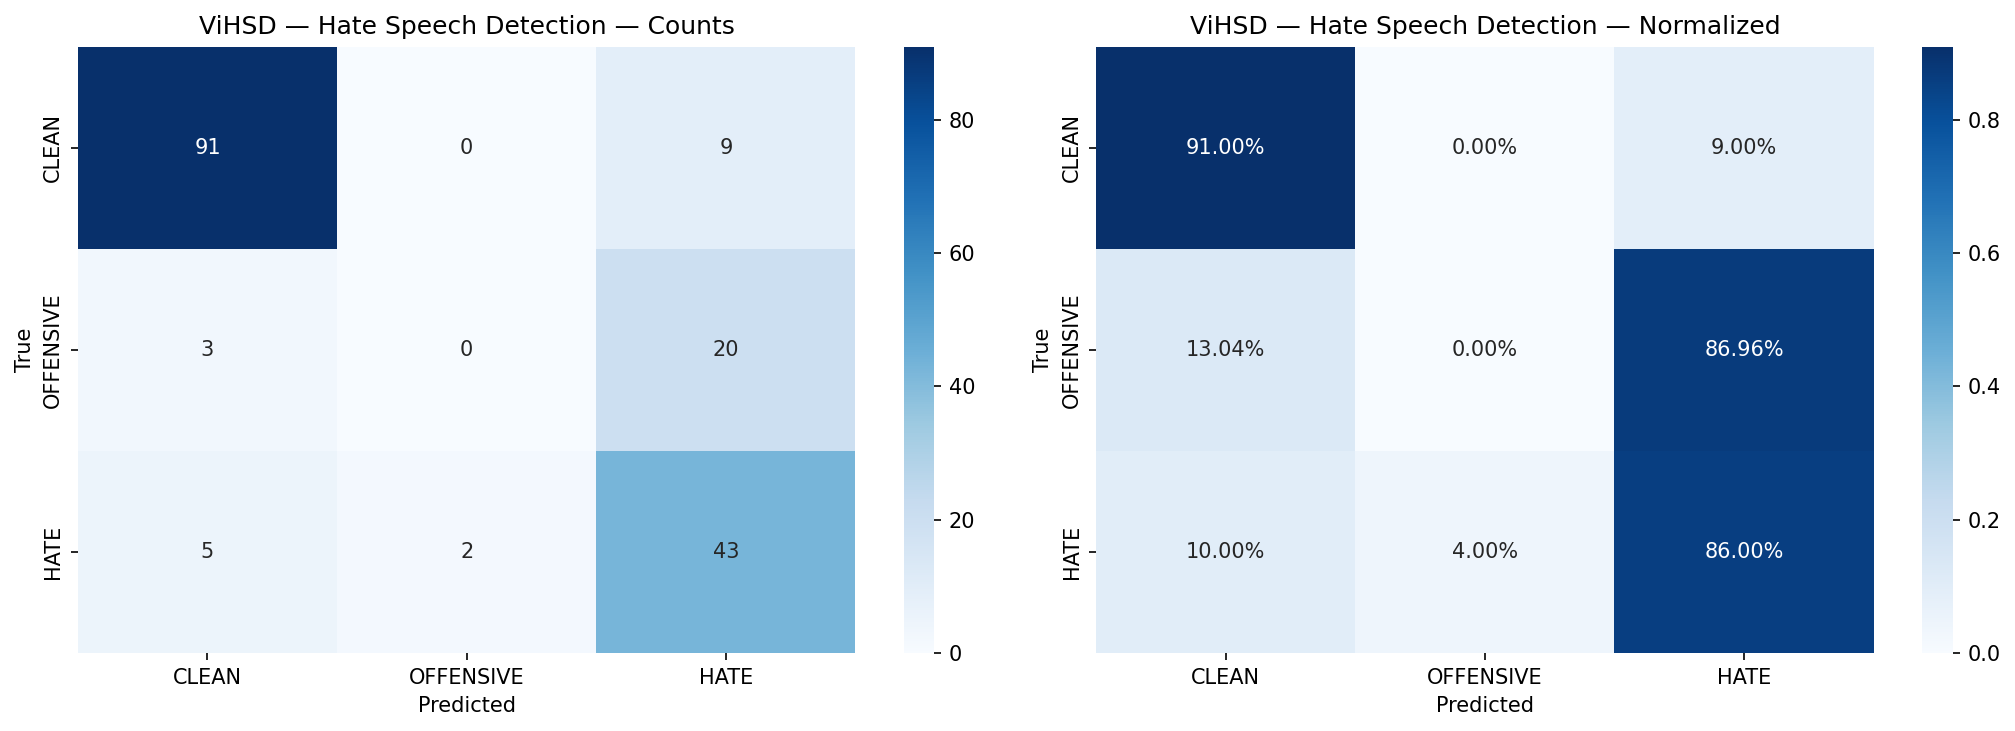
\includegraphics[width=\linewidth]{confusion_matrix_vihsd_vit5_finetune_multi.png}
\caption{ViT5 multi-task.}
\end{subfigure}
\hfill
\begin{subfigure}{0.32\textwidth}
\centering
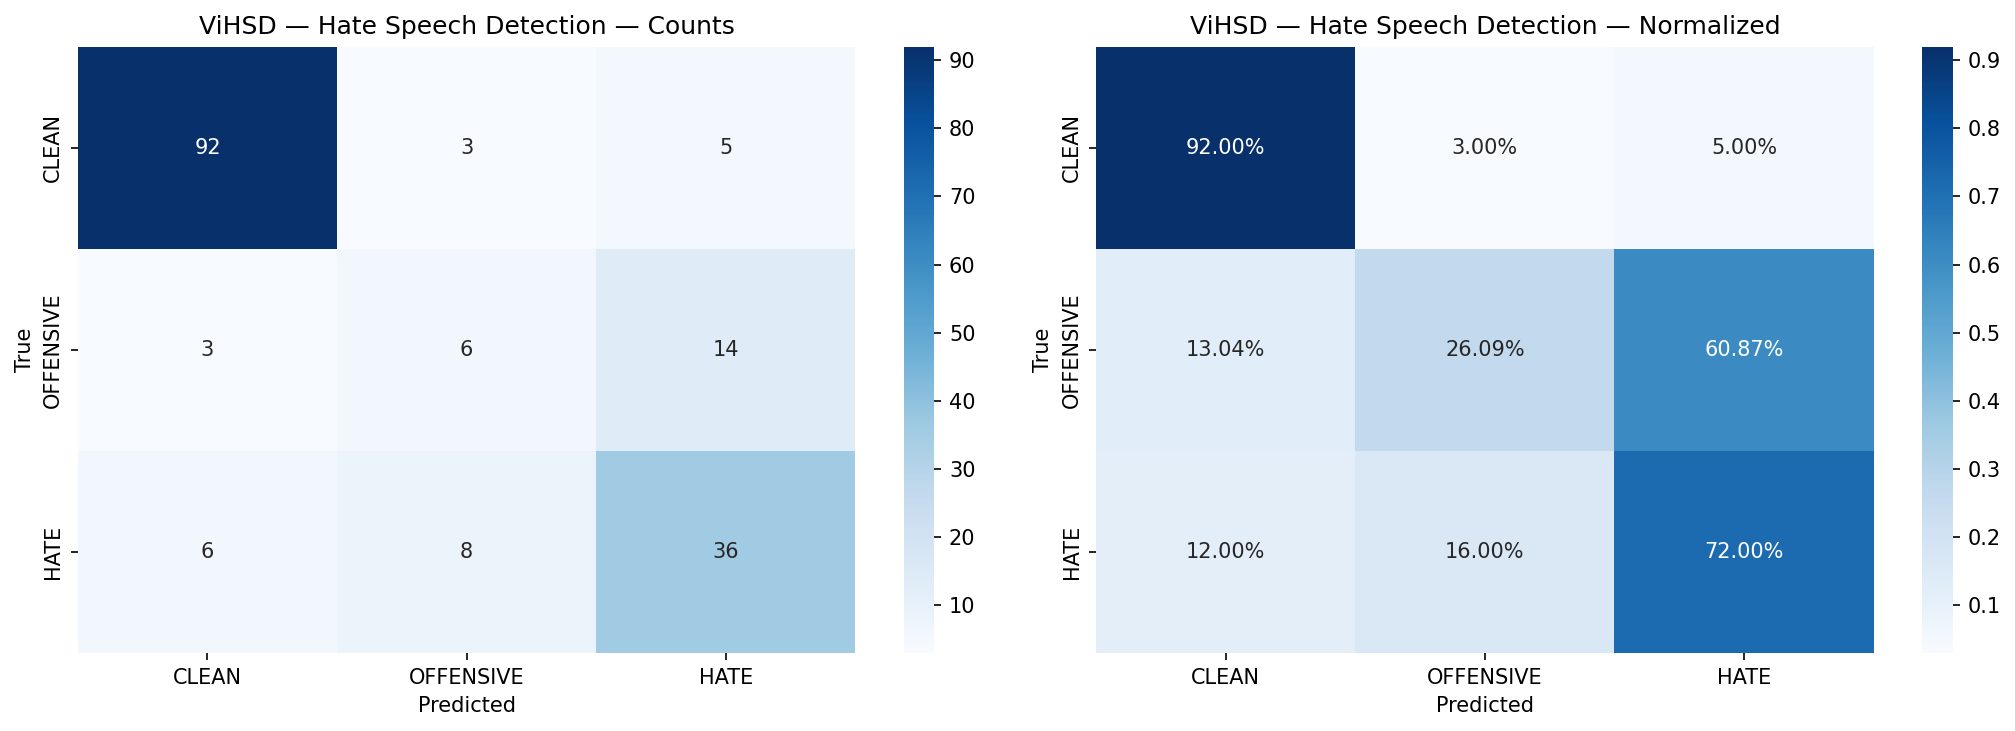
\includegraphics[width=\linewidth]{confusion_matrix_vihsd_vit5_finetune_hate_only.png}
\caption{ViT5 hate-only.}
\end{subfigure}
\hfill
\begin{subfigure}{0.32\textwidth}
\centering
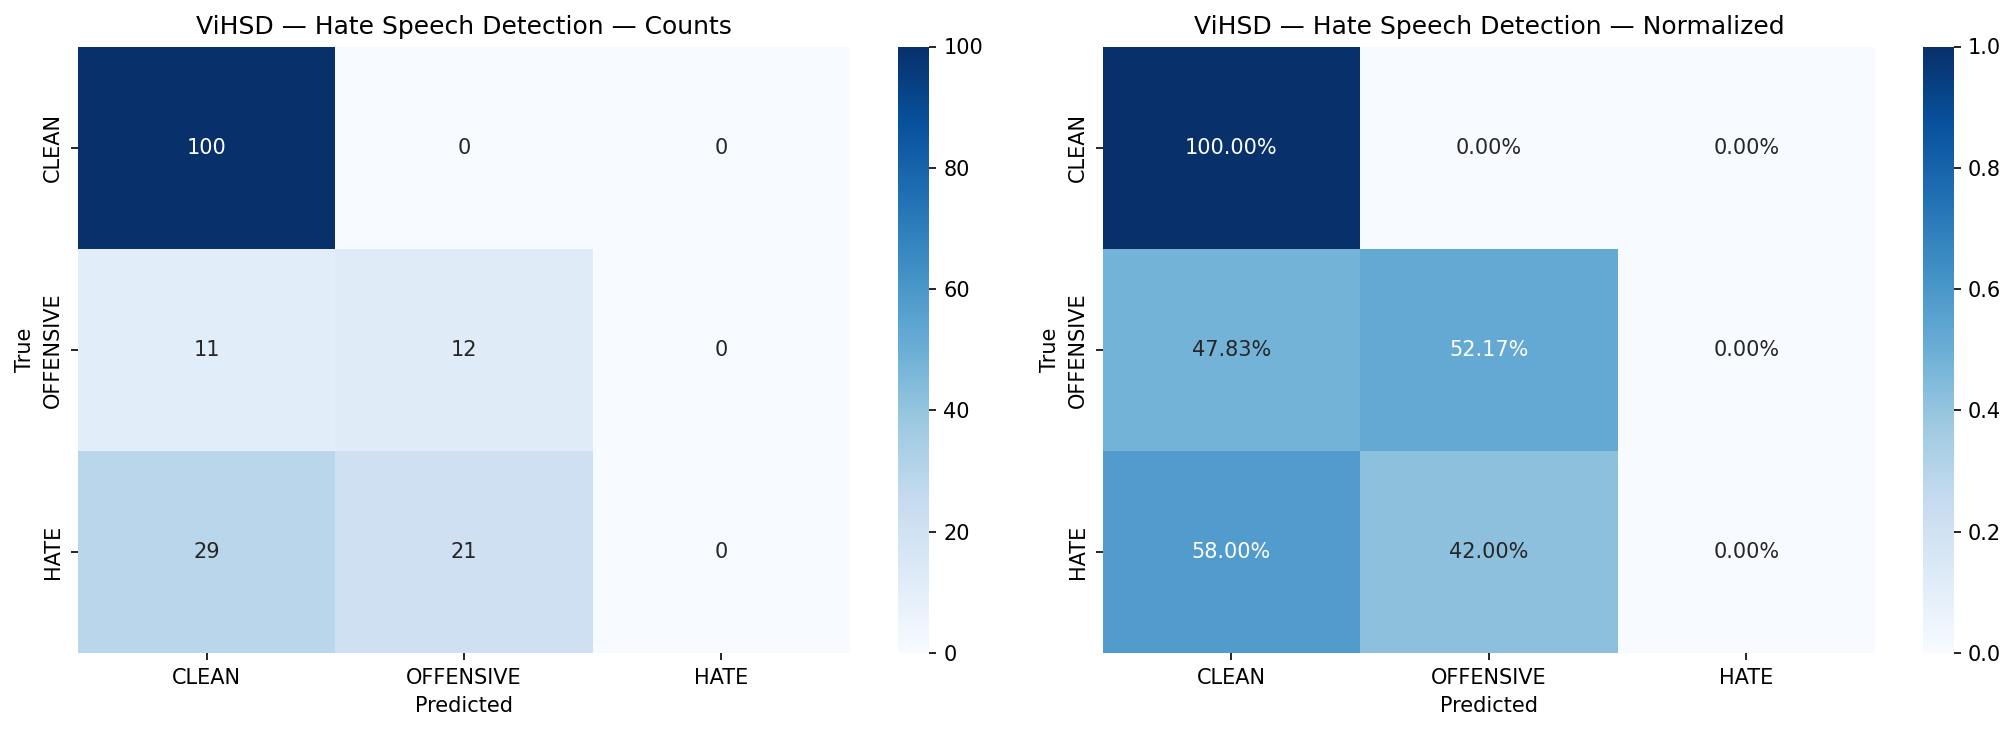
\includegraphics[width=\linewidth]{confusion_matrix_vihsd_visobert_labeling.png}
\caption{ViSoBERT labeling.}
\end{subfigure}
\vspace{0.4em}

\begin{subfigure}{0.32\textwidth}
\centering
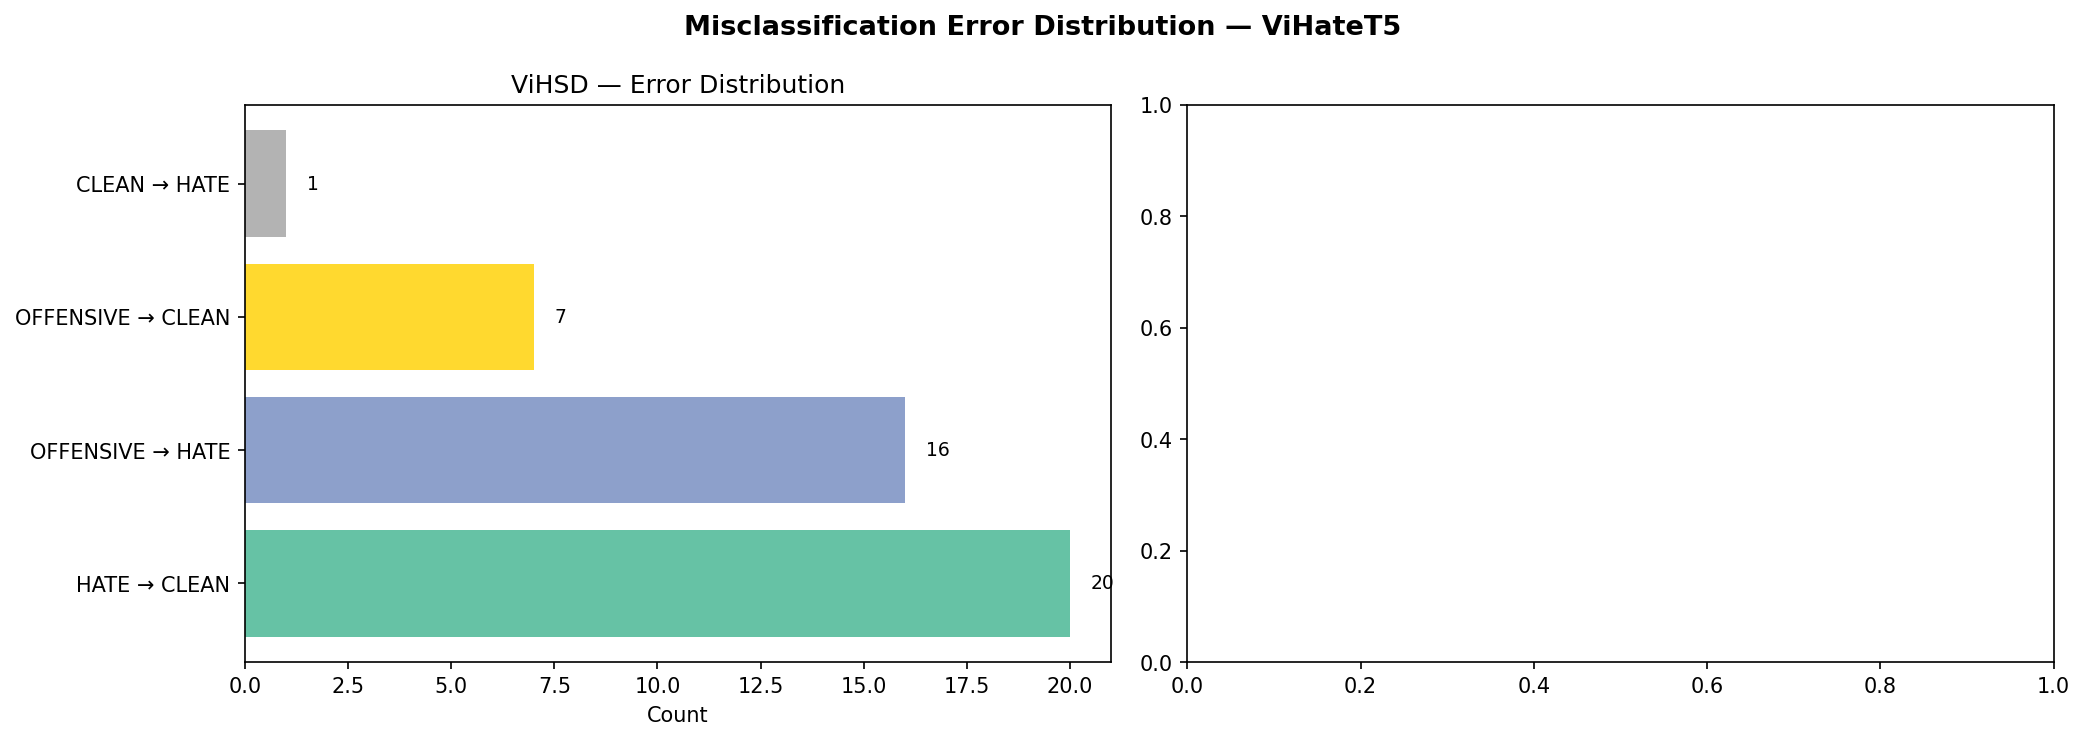
\includegraphics[width=\linewidth]{error_distribution_vit5_focal_loss_exp.png}
\caption{Focal Loss.}
\end{subfigure}
\hfill
\begin{subfigure}{0.32\textwidth}
\centering
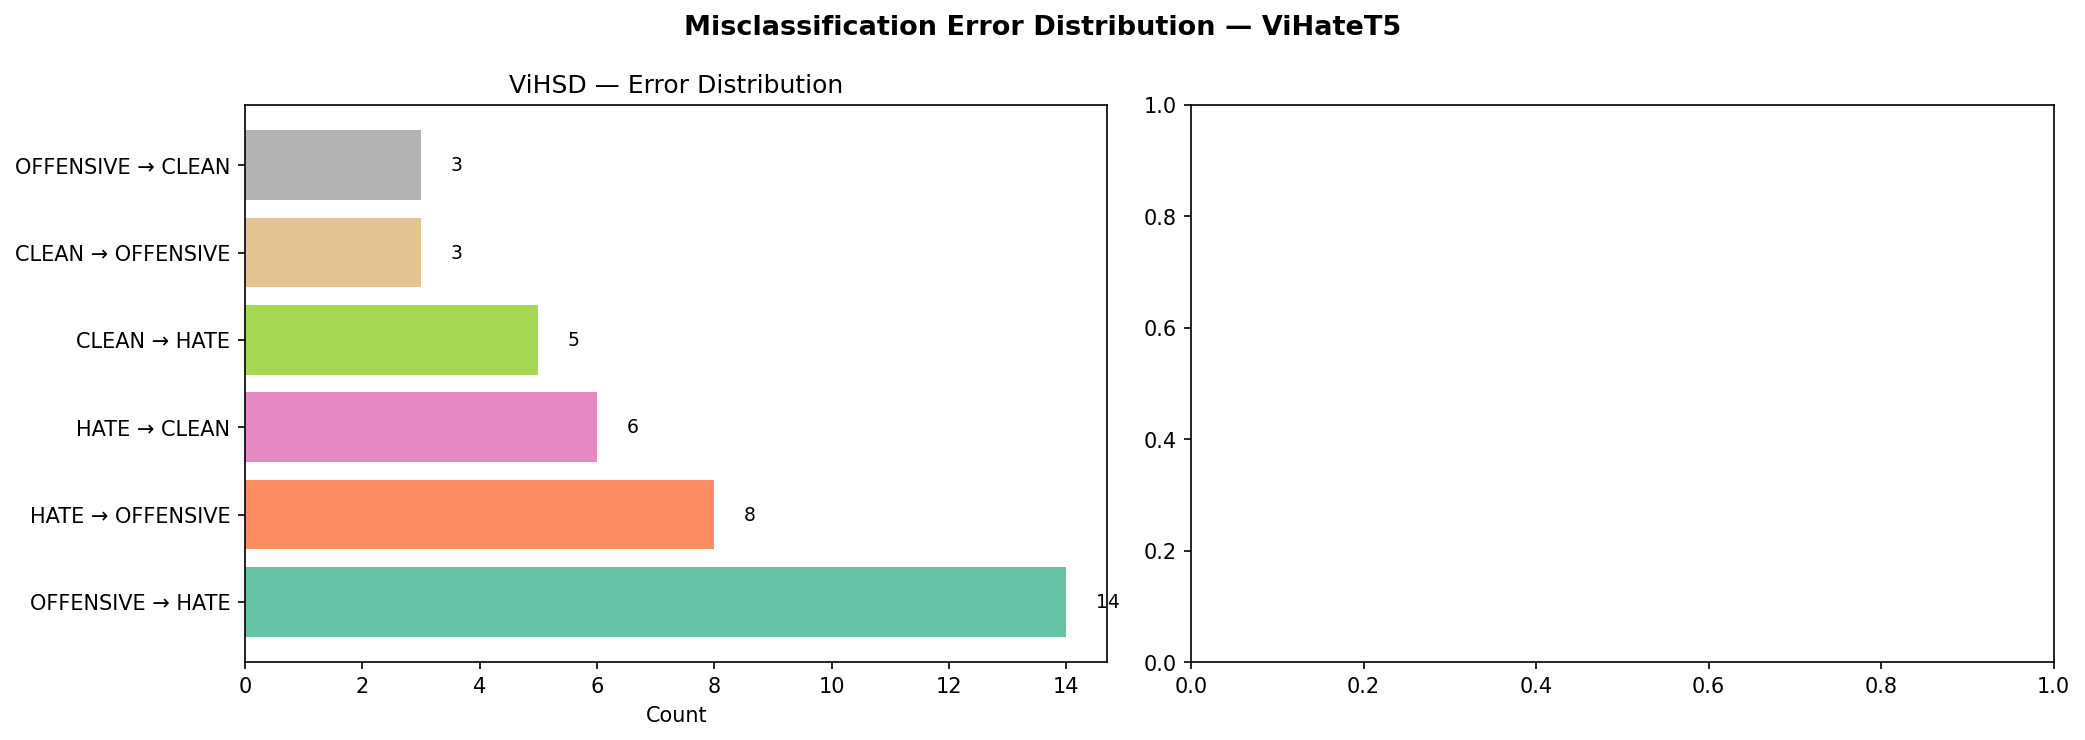
\includegraphics[width=\linewidth]{error_distribution_vit5_finetune_hate_only.png}
\caption{Hate-only.}
\end{subfigure}
\hfill
\begin{subfigure}{0.32\textwidth}
\centering
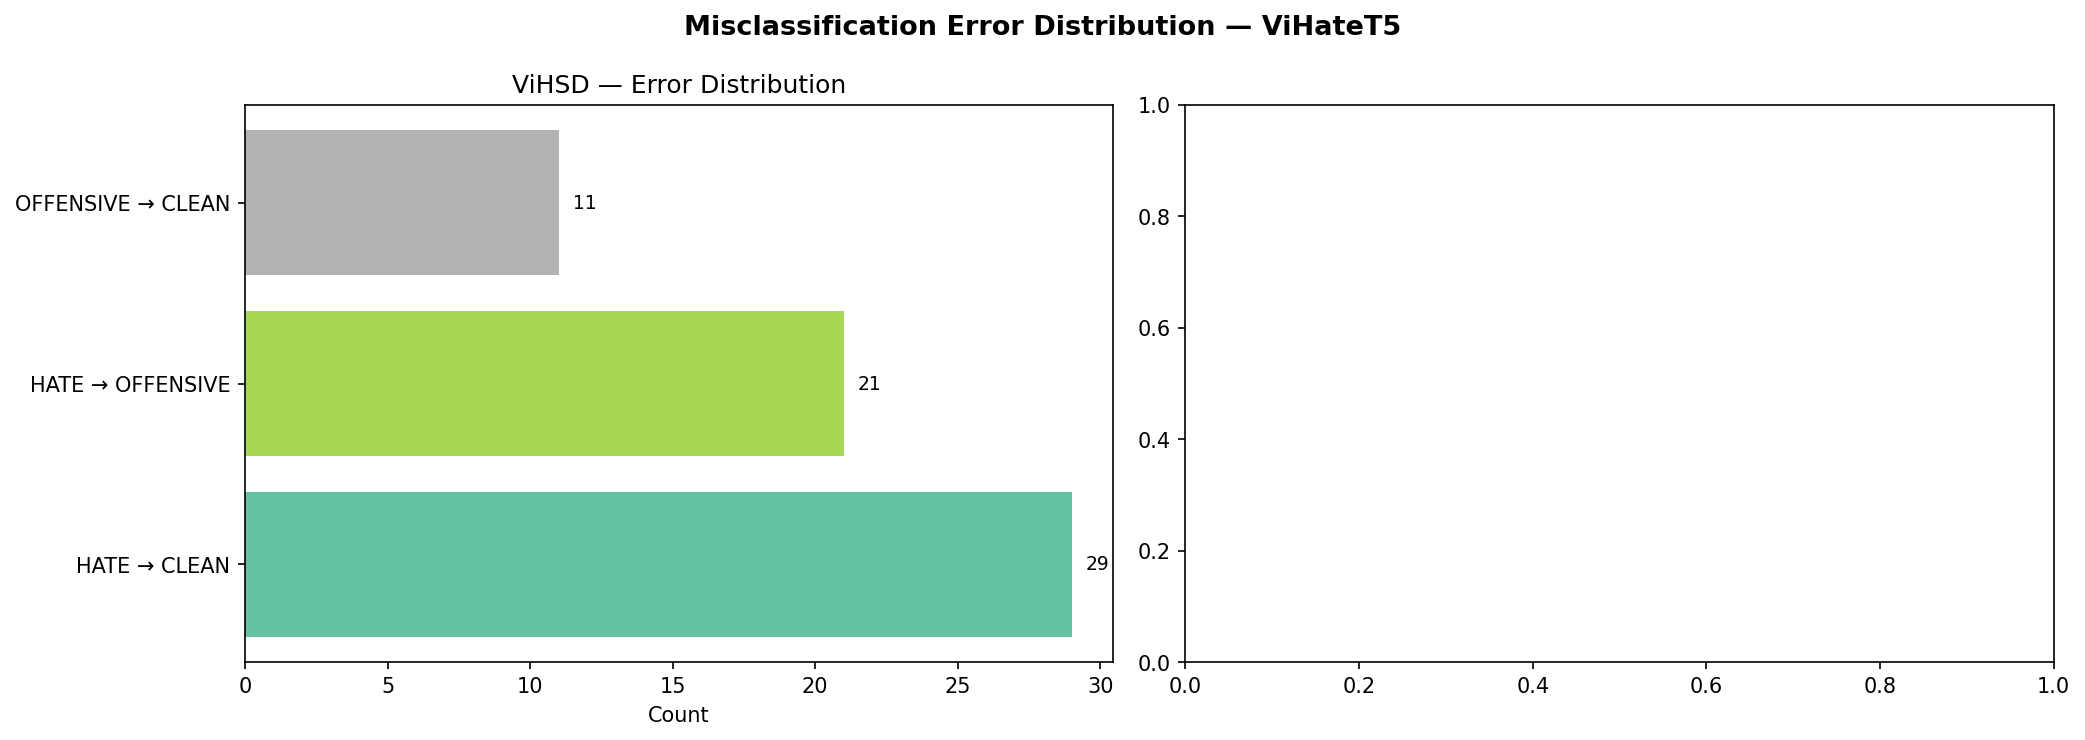
\includegraphics[width=\linewidth]{error_distribution_visobert_labeling.png}
\caption{ViSoBERT.}
\end{subfigure}
\caption{Additional diagnostic figures for ViHSD. The first row shows confusion matrices for ViT5 multi-task, ViT5 hate-only, and ViSoBERT labeling. The second row shows the corresponding error-distribution charts for Focal Loss, hate-only, and ViSoBERT.}
\label{fig:appendix_extra}
\end{figure*}

Figure \ref{fig:appendix_extra} compares additional confusion matrices beyond the two representative models in the main text. The ViT5 multi-task variant correctly recognizes most CLEAN comments: 91 out of 100 CLEAN samples are predicted as CLEAN. However, it almost never predicts OFFENSIVE correctly. In the OFFENSIVE row, 20 out of 23 OFFENSIVE samples are predicted as HATE, while none are predicted as OFFENSIVE. This means the model learns that these comments are harmful, but it does not learn the finer boundary between offensive language and hate speech. The HATE class is also detected reasonably well, with 43 out of 50 HATE samples predicted as HATE, but a few HATE samples are still softened into CLEAN or OFFENSIVE.

The hate-only variant behaves differently. It still recognizes CLEAN well, with 92\% of CLEAN examples classified correctly, but it becomes more willing to use the OFFENSIVE label than the multi-task variant. For OFFENSIVE, it correctly predicts 6 out of 23 samples, while 14 are still pushed into HATE. For HATE, it correctly predicts 36 out of 50 samples, but 8 are predicted as OFFENSIVE and 6 as CLEAN. This suggests that hate-only pre-training increases sensitivity to harmful content, but it does not fully solve class separation. It improves attention to toxic patterns, yet the distinction between OFFENSIVE and HATE remains unstable.

The ViSoBERT labeling model shows another extreme behavior. It correctly predicts all 100 CLEAN samples as CLEAN, but it never predicts the HATE column in this confusion matrix. OFFENSIVE samples are split between CLEAN and OFFENSIVE, with 12 out of 23 predicted as OFFENSIVE and 11 as CLEAN. HATE samples are distributed into CLEAN and OFFENSIVE, with 29 predicted as CLEAN and 21 as OFFENSIVE. This is consistent with the role of ViSoBERT in the project: it is strong as a social-media encoder and useful for binary auto-labeling, but its label mapping is not ideal for the full three-class ViHSD setting. Therefore, this figure supports the decision to use ViSoBERT mainly as an auto-labeling component rather than as the final unified three-task model.

The second row of Figure \ref{fig:appendix_extra} shows the same story from the perspective of error types rather than full confusion matrices. For the Focal Loss model, the largest error type is HATE $\rightarrow$ CLEAN, with 20 cases. This means that although Focal Loss improves the aggregate ViHSD \mf{} in Table \ref{tab:focal}, it still misses a significant number of true HATE comments by classifying them as CLEAN. The second-largest error type is OFFENSIVE $\rightarrow$ HATE, with 16 cases. This indicates that Focal Loss pushes many borderline offensive comments toward the more severe HATE label. In practice, this can be risky: over-flagging offensive comments as hate speech may increase false alarms, while HATE $\rightarrow$ CLEAN mistakes may let genuinely harmful content pass through.

For the hate-only model, the dominant error is OFFENSIVE $\rightarrow$ HATE, with 14 cases. This is expected because hate-only pre-training exposes the model heavily to harmful expressions. As a result, when it sees offensive language, it tends to interpret it as hate speech. The next important error is HATE $\rightarrow$ OFFENSIVE, with 8 cases, followed by HATE $\rightarrow$ CLEAN with 6 cases and CLEAN $\rightarrow$ HATE with 5 cases. Compared with Focal Loss, the hate-only variant spreads errors across more directions, but its strongest bias is still toward confusing OFFENSIVE and HATE. This confirms that simply increasing exposure to hate-like patterns does not automatically teach the model the semantic boundary between an individual insult and a group-targeted hateful statement.

For ViSoBERT, the error distribution is much more concentrated. The largest bar is HATE $\rightarrow$ CLEAN, with 29 cases, followed by HATE $\rightarrow$ OFFENSIVE, with 21 cases, and OFFENSIVE $\rightarrow$ CLEAN, with 11 cases. This means ViSoBERT often downgrades harmful content instead of predicting the strongest harmful class. From a moderation perspective, this is a false-negative problem: the model may be conservative and avoid assigning HATE. This behavior is acceptable for some auto-labeling uses if the goal is to generate a broad clean/harmful split, but it is weaker for final three-class classification. Overall, Figure \ref{fig:appendix_extra} justifies why the report does not rely only on average \mf{}. A model can score well in one aggregate metric while still having an undesirable error profile for moderation.

\clearpage

\begin{thebibliography}{99}
\bibitem{vihatet5}
L. T. Nguyen, ``ViHateT5: Enhancing Hate Speech Detection in Vietnamese With a Unified Text-to-Text Transformer Model,'' in \emph{Findings of the Association for Computational Linguistics: ACL}, 2024, pp. 5948--5961.

\bibitem{t5}
C. Raffel \emph{et al.}, ``Exploring the Limits of Transfer Learning with a Unified Text-to-Text Transformer,'' \emph{Journal of Machine Learning Research}, vol. 21, no. 140, pp. 1--67, 2020.

\bibitem{mt5}
L. Xue \emph{et al.}, ``mT5: A Massively Multilingual Pre-trained Text-to-Text Transformer,'' in \emph{Proc. NAACL}, 2021.

\bibitem{vit5}
L. Phan, H. Tran, H. Nguyen, and T. Nguyen, ``ViT5: Pretrained Text-to-Text Transformer for Vietnamese Language Generation,'' in \emph{Proc. COLING}, 2022, pp. 4029--4041.

\bibitem{phobert}
D. Q. Nguyen and A. T. Nguyen, ``PhoBERT: Pre-trained Language Models for Vietnamese,'' in \emph{Findings of EMNLP}, 2020, pp. 1037--1042.

\bibitem{visobert}
N. Nguyen \emph{et al.}, ``ViSoBERT: A Pre-trained Language Model for Vietnamese Social Media Text Processing,'' in \emph{Proc. EMNLP}, 2023, pp. 5191--5207.

\bibitem{hatebert}
T. Caselli, V. Basile, J. Mitrovic, and M. Granitzer, ``HateBERT: Retraining BERT for Abusive Language Detection in English,'' in \emph{Proc. WOAH}, 2021.

\bibitem{vihsd}
S. T. Luu \emph{et al.}, ``A Large-scale Dataset for Hate Speech Detection on Vietnamese Social Media Texts,'' in \emph{Proc. IEA/AIE}, 2021, pp. 415--426.

\bibitem{victsd}
P. G. Hoang \emph{et al.}, ``Constructive and Toxic Speech Detection for Open-domain Social Media Comments in Vietnamese,'' in \emph{Proc. IEA/AIE}, 2021, pp. 572--583.

\bibitem{vihos}
P. G. Nguyen \emph{et al.}, ``ViHOS: Hate Speech Spans Detection for Vietnamese,'' in \emph{Proc. EACL}, 2023, pp. 652--669.

\bibitem{focalloss}
T.-Y. Lin, P. Goyal, R. Girshick, K. He, and P. Dollar, ``Focal Loss for Dense Object Detection,'' in \emph{Proc. ICCV}, 2017, pp. 2980--2988.

\bibitem{eda}
J. W. Wei and K. Zou, ``EDA: Easy Data Augmentation Techniques for Boosting Performance on Text Classification Tasks,'' in \emph{Proc. EMNLP-IJCNLP Workshop}, 2019.
\end{thebibliography}

\begin{IEEEbiography}[{\includegraphics[width=1in,height=1.25in,clip,keepaspectratio]{member1.jpg}}]{Nguyen Cong Phat}
is a third-year Computer Science student specializing in Artificial Intelligence and Data Analysis. He currently serves as an AI Engineer at KMS Technology Vietnam. He has experience solving applied problems in Natural Language Processing, Computer Vision, and data-driven system design. His interests include transformer-based language models, Vietnamese social-media text processing, model evaluation, and practical deployment of machine learning systems. In this project, he contributed to the reimplementation of ViHateT5, experimental analysis, result interpretation, and report preparation.
\end{IEEEbiography}

\begin{IEEEbiography}[{\includegraphics[width=1in,height=1.25in,clip,keepaspectratio]{member2.jpg}}]{Vu Viet Cuong}
is a third-year Computer Science student specializing in Artificial Intelligence and Data Analysis. He has experience solving applied problems in Natural Language Processing, Computer Vision, and data-driven system design. His interests include transformer-based language models, Vietnamese social-media text processing, model evaluation, and practical deployment of machine learning systems. In this project, he contributed to data processing, baseline model experiments, result visualization, and analysis of Vietnamese hate speech detection benchmarks.
\end{IEEEbiography}

\begin{IEEEbiography}[{\includegraphics[width=1in,height=1.25in,clip,keepaspectratio]{member3.jpg}}]{Truong Hoang Thanh An}
is a third-year Computer Science student specializing in Artificial Intelligence and Data Analysis. He has experience solving applied problems in Natural Language Processing, Computer Vision, and data-driven system design. His interests include transformer-based language models, Vietnamese social-media text processing, model evaluation, and practical deployment of machine learning systems. In this project, he contributed to model training, improvement experiments, web demonstration, and repository organization for reproducible evaluation.
\end{IEEEbiography}

\end{document}
